% !TEX encoding = UTF-8

%% Davide Imola - VR386238
%% Andre Slemer - VR386253
%% Giovanni Bellorio - VR386665
%% Esame di LaTeX

\documentclass[a4paper,titlepage]{book}

\usepackage[italian]{babel}
\usepackage[nowrite,noadvisor]{frontespizio}
\usepackage{amsmath,amssymb,graphicx}
\usepackage{natbib}
\usepackage{url}
\usepackage{float}

\begin{document}

\pagestyle{plain}

%Generazione Frontespizio
\begin{frontespizio}
\Universita{Verona}
\Dipartimento{Informatica}
\Corso[Laurea]{Informatica}
\Annoaccademico{2016--2017}
\Titoletto{Ingegneria del Software}
\Titolo{Documento dei Requisiti}
\Sottotitolo{Negozio CD musicali}
\Candidato[VR386253]{Andrea Slemer}
\Candidato[VR386238]{Davide Imola}
\Candidato[VR386665]{Giovanni Bellorio}
\end{frontespizio}

\frontmatter
\tableofcontents

\mainmatter
\chapter{Testo elaborato}
Si vuole progettare un sistema informativo per gestire le informazioni relative alla gestione di un negozio
virtuale di CD e DVD musicali (vende solo via web).
Il negozio mette in vendita CD di diversi generi: jazz, rock, classica, latin, folk, world-music, e cos\`i via.
Per ogni CD o DVD il sistema memorizza: un codice univoco, il titolo, i titoli di tutti i pezzi contenuti,
eventuali fotografie della copertina, il prezzo, la data dalla quale \`e presente sul sito web del negozio, il
musicista/band titolare, una descrizione, il genere del CD o DVD, i musicisti che vi suonano, con il
dettaglio degli strumenti musicali usati. Per ogni musicista il sistema registra il nome d’arte, il genere
principale, l’anno di nascita, se noto, gli strumenti che suona.
Sul sito web del negozio \`e illustrato il catalogo dei prodotti in vendita.
Cliccando sul nome del prodotto, appare una finestra con i dettagli del prodotto stesso.
I clienti possono acquistare on-line selezionando gli oggetti da mettere in un “carrello della spesa”
virtuale.
Deve essere possibile visualizzare il contenuto del carrello, modificare il contenuto del carrello, togliendo
alcuni articoli.
Al termine dell’acquisto va gestito il pagamento, che pu\`o avvenire con diverse modalit\`a.
Il sistema supporta differenti ricerche: per genere, per titolare del CD o DVD, per musicista partecipante,
per prezzo. Coerentemente, differenti modalit\`a di visualizzazione, sono altres\`i supportate.
Ogni vendita viene registrata indicando il cliente che ha acquistato, i prodotti acquistati, il prezzo
complessivo, la data di acquisto, l’ora, l’indirizzo IP del PC da cui \`e stato effettuato l’acquisto, la modalit\'a
di pagamento (bonifico, carta di credito, paypal) e la modalit\`a di consegna (corriere, posta, ...).
Per ogni cliente il sistema registra: il suo codice fiscale, il nome utente (univoco) con cui si \`e registrato,
la sua password, il nome, il cognome, la citt\`a di residenza, il numero di telefono ed eventualmente il
numero di cellulare.
Per i clienti autenticati, il sistema propone pagine specializzate che mostrano suggerimenti basati sul
genere dei precedenti prodotti acquistati.
Se il cliente ha fatto gi\`a 3 acquisti superiori ai 250 euro l’uno entro l’anno, il sistema gli propone sconti e
consegna senza spese di spedizione.
Il personale autorizzato del negozio pu\`o inserire tutti i dati dei CD e DVD in vendita. Il personale
inserisce anche il numero di pezzi a magazzino. Il sistema tiene aggiornato il numero dei pezzi a
magazzino durante la vendita e avvisa il personale del negozio quando un articolo (CD o DVD) scende
sotto i 2 pezzi presenti in magazzino.

\chapter{Idee di progettazione}
\section{Generale}
Abbiamo progettato un'applicazione Java che si interfaccia ad un server Postgres per l'acquisizione e
l'immagazzinamento dei dati. L'applicazione prevede un'interfaccia che permette di soddisfare le richieste
di due categorie di utenti:
\begin{itemize}
\item CLIENTI: i quali avranno la possibilit\`a di acquistare CD/DVD dal negozio online
\item PERSONALE: il quale avr\'a la possibili\`a di gestire il magazzino modificando dati nel database attraverso un GUI
\end{itemize}

\section{Versione attuale}
In questa versione dell'applicazione ci siamo concentrati nello sviluppo dell'interfaccia lato cliente.
L'utente avr\`a la possibilit\`a di sfogliare il catalogo con i prodotti, ottenere informazioni dettagliate per un prodotto
specifico, connettersi con un proprio account personale per effettuare acquisti, potendo modificare il contenuto 
del proprio carrello virtuale e visualizzare gli ordini gi\`a effettuati con tale account. Inoltre sar\`a possibilie creare un nuovo account qualora l'utente non dovesse disporne di uno.

\subsection{Database -  PostGres}
Il catalogo dei cd/dvd disponibili nello store viene visualizzato interrogando la base di dati. La tabella che contiene le informazioni necessarie \`e Disco, identificata univocamente da un un id auto incrementante. La tabella Disco contiene il titolo, il prezzo, la data di inserimento, una descrizione breve, la quantit\`a disponibile e una foto relativa all'oggetto. Le informazioni relative al genere, all'artista e ai musicisti interpreti nel cd/dvd vengono registrati separatemente in altre tabelle per evitare ridondanza nei dati. Si accede alle tabelle di Genere, Artista, Musicista tramite query Join. Per registrare anche gli strumenti suonati dall'artista e dai musicisti si accede alla tabella Suona per i musicisti, alla tabella artista musicista per gli artisti. Gli artisti, i musicisti e gli strumenti vengono registrati con un id auto incrementate e il loro relativo nome. Tutte le informazioni da aggiungere al catalogo e non presenti nella tabella Disco vengono reperite attraverso join con id di tabelle.
Il nostro sistema prevede solamente la visualizzazione degli strumenti suonati nel cd da parte di artisti o musicisti. La base di dati memorizza anche tutti gli strumenti suonati da un artista o musicista.
La parte sinistra della base di dati prevede la memorizzazione dei carrelli e la storia degli ordini per ogni cliente. Il cliente viene registrato con codice univoco auto incrementante, user id, password, codice fiscale, nome, cognome, città di residenza, telefono e cellulare. Il carrello viene associato all'id del cliente qualora si aggiunga un cd/dvd. L'inserimento prevede l'associazione id disco e id cliente. Il carrello rimane memorizzato nella tabella fino a ordine avvenuto con successo. Un ordine viene identificato da un id auto incrementante, dal costo totale, dalla data, ora, modalit\`a pagamento e consegna. L'ordine come il carrello viene associato all'id disco e all'id cliente. L'ordine rimane memorizzato per mantenere la storia totale.

\subsection{GUI -  Java}
La parte grafica del prototipo \`e stata implementata estendendo le classi con JFrame scrivendo codice puro senza nessun supporto di visualizzazione grafico. Per offrire interattivit\`a utente-sistema sono stati inseriti JTextField e anche JRadioButton. L'architettura utilizzata nell'applicazione \`e quella Model-View-Control (MVC). La classe view principale visualizza direttamente il catalogo senza dover eseguire nessuna autenticazione. La visualizzazione del catalogo viene eseguita inserendo i dati in una tabella senza righe e colonne posizionando i dati in un array che viene inserito direttamente nella tabella. Le informazioni relative ad un disco vengono ottenute selezionando la riga del disco nella tabella implementando un evento di ascolto. Viene eseguita una navigazione tra le varie pagine grazie all'inserimento di bottoni sui quali viene configurato un evento di ascolto che fa comparire la nuova pagine ed elimina la precedente. Per il login e la registrazione abbiamo pensato ad una versione pop-up realizzando due finestre di dimensione diversa e sovrapposte senza cancellare quello gi\`a fatto all'interno dell'applicazione. Le classi Carrello e Ordini funzionano in modo simile alla classe Catalogo interrogando la base di dati correttamente attraverso la classe Model e ottenendo i risultati all'interno di una tabella sotto-forma di array. La classe ModalitaOrdine offre la possibilit\`a di inserire diverse modalit\`a di ordine del cliente tramite un JRadioButton. La classe Pagamento \`e di collegamento: il server restituisce le coordinate bancarie per l'eventuale bonifico oppure richiede il codice della carta di credito, oppure email e password per il collegamento a PayPal. Effettuato il pagamento si transita alla pagina ordini. La classe login prevede l'inserimento dell'user id e della password. La password viene inserita in un JPasswordField, il quale permette una scrittura segreta, dal quale si estraggono i singoli caratteri decodificati. Inoltre per offrire maggior sicurezza la password viene criptata con un algoritmo di cifratura MD5 implementato in un metodo Java nel model.
La registrazione prevede l'inserimento di tutte le informazioni del cliente con controlli sulla lunghezza del codice fiscale e degli altri campi. Una volta effettuato il login viene visualizzato il nome di accesso reperito grazie al salvataggio dell'user id inserito in una variabile pubblica statica.

\chapter{Metodo di sviluppo}
La versione attuale dell'applicazione \`e stata implementata usando un metodo di progettazione agile, cercando similitudini e 
facendo confronti con i pi\`u famosi siti di e-commerce. Abbiamo organizzato il lavoro in modo da essere sempre efficenti utilizzando Git un software di controllo versione distribuito.\\
Grazie a questa piattaforma abbiamo potuto alternare scrittura di codice da casa ad incontri regolari in universit\'a per organizzare
le idee, confrontarsi, dividersi i compiti e darci delle scadenze ai lavori assegnatici.\\
Con GitHub abbiamo potuto tenere ben separati modelli sperimentali e non ancora testati, scritti e documentati su un branch developer, e i modelli che hanno superato la fase di testing, sul branch master.\\
In questo modo ci \`e sempre stato possibile fare un confronto per l'aggiornamento della nuova versione dell'applicazione,
e nel caso ne avessimo avuto necessit\`a la possibilit\`a di avere sempre una versione affidabile di partenza per un eventuale rollback.

\chapter{Requisiti}
\section{Requisiti funzionali}
\subsection{Caso d'uso 1}
\begin{itemize}
\item Sull'applicazione del negozio \`e illustrato il catalogo dei prodotti in vendita.
\item Cliccando sul nome dello strumento la finestra permette la visualizzazione dei dettagli del CD/DVD selezionato.
\item L'applicazione supporta diverse ricerche: genere, titolare del CD o DVD, musicista partecipante, prezzo.
\end{itemize}
Vengono generati lo Use Case \figurename~\ref{fig:use1} e i Sequence Diagram \figurename~\ref{fig:seq1f} e \figurename~\ref{fig:seq1b}.

\subsection{Caso d'uso 2}
\begin{itemize}
\item I clienti effettuare degli acquisti selezionando gli oggetti da mettere in un carrello virtuale.
\item \`E possibile visualizzare il contenuto del carrello, modificandone il contenuto, aggiungendo o togliendo alcuni articoli.
\item Al termine dell'acquisto viene gestito il pagamento, che pu\`o avvenire attraverso tre diverse modalit\`a.
\end{itemize}
Vengono generati lo Use Case \figurename~\ref{fig:use2} e i Sequence Diagram \figurename~\ref{fig:seq2f} e \figurename~\ref{fig:seq2b}.

\subsection{Caso d'uso 3}
\begin{itemize}
\item Tutti i clienti possono registrarsi al sito per effettuare acquisti.
\item I clienti autenticati ricevono pagine specializzate con prodotti consigliati, rispetto agli oggetti precedentemente acquistati.
\item Se il cliente ha gi\`a fatto tre acquisti superiori ai 250 euro l'un entro l'anno, il sistema propone ulteriori sconti e consegna senza spese di spezione.
\end{itemize}
Vengono generati lo Use Case \figurename~\ref{fig:use3} e i Sequence Diagram \figurename~\ref{fig:seq3f} e \figurename~\ref{fig:seq3b}.

\subsection{Caso d'uso 4}
\begin{itemize}
\item Il personale pu\`o inserire i dati per nuovi CD o DVD da mettere in vendita.
\item Il personale pu\`o aggiornare il numero di pezzi in magazzino per i CD/DVD in vendita.
\item Il personale viene avvisato se un oggetto del catalogo scende sotto i 2 pezzi in magazzino.
\end{itemize}
Vengono generati lo Use Case \figurename~\ref{fig:use4} e i Sequence Diagram \figurename~\ref{fig:seq4f1} e \figurename~\ref{fig:seq4f2}.

\section{Requisiti di dominio}
Dato il testo dei requisti sono stati estrapolati i seguenti vincoli per le tabelle:
\begin{itemize}
\item CD/DVD \\
codice univoco, titolo, titoli di tutti i pezzi contenuti, eventuali foto copertina, prezzo, data presenza sul sito, musicista/band titolare. descrizione, genere del CD o DVD, musicisti che vi suonano con dettaglio su strumenti musicali usati, quantit\`a

\item GRUPPO \\
id, nome, genere principale, anno di fond (opzionale), lista musicisti

\item MUSICISTA \\
id, Nome d’arte, genere principale, anno di nascita (opzionale) se noto e strumenti

\item ORDINE \\
numero ordine, Cliente, lista prodotti, prezzo complessivo, data acquisto, ora, indirizzo IP del PC, modalit\`a di pagamento (bonifico, carta, paypal), modalit\`a di consegna (corriere, posta, ….)

\item CLIENTE \\
codice fiscale, nome utente (univoco), password, nome, cognome, città residenza, numero telefono, numero cellulare (opzionale)
\end{itemize}

\chapter{Diagrammi}
\section{Use Case}
\begin{figure}[H]
\center
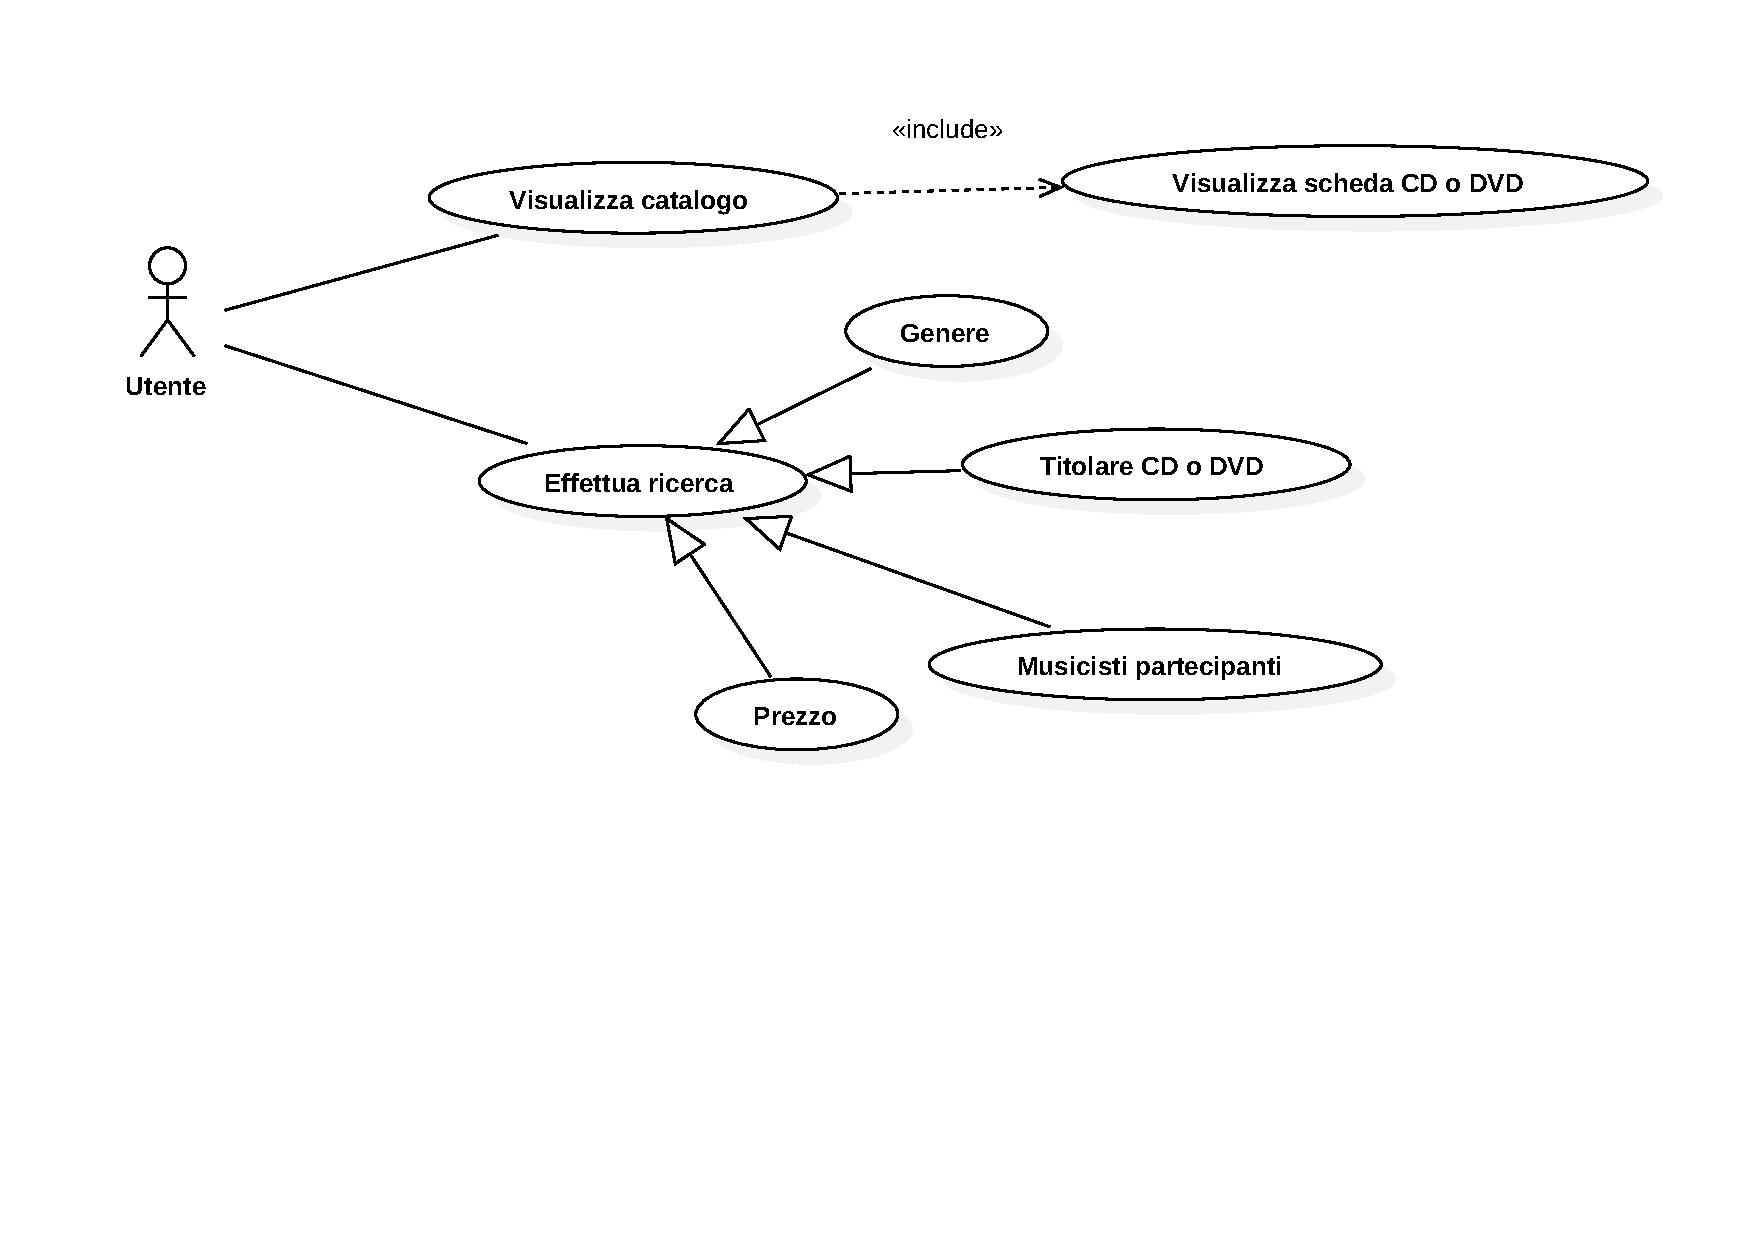
\includegraphics[width=350px]{img/Use1.pdf}
\caption{Use Case 1 \label{fig:use1}}
\end{figure}
\begin{figure}[H]
\center
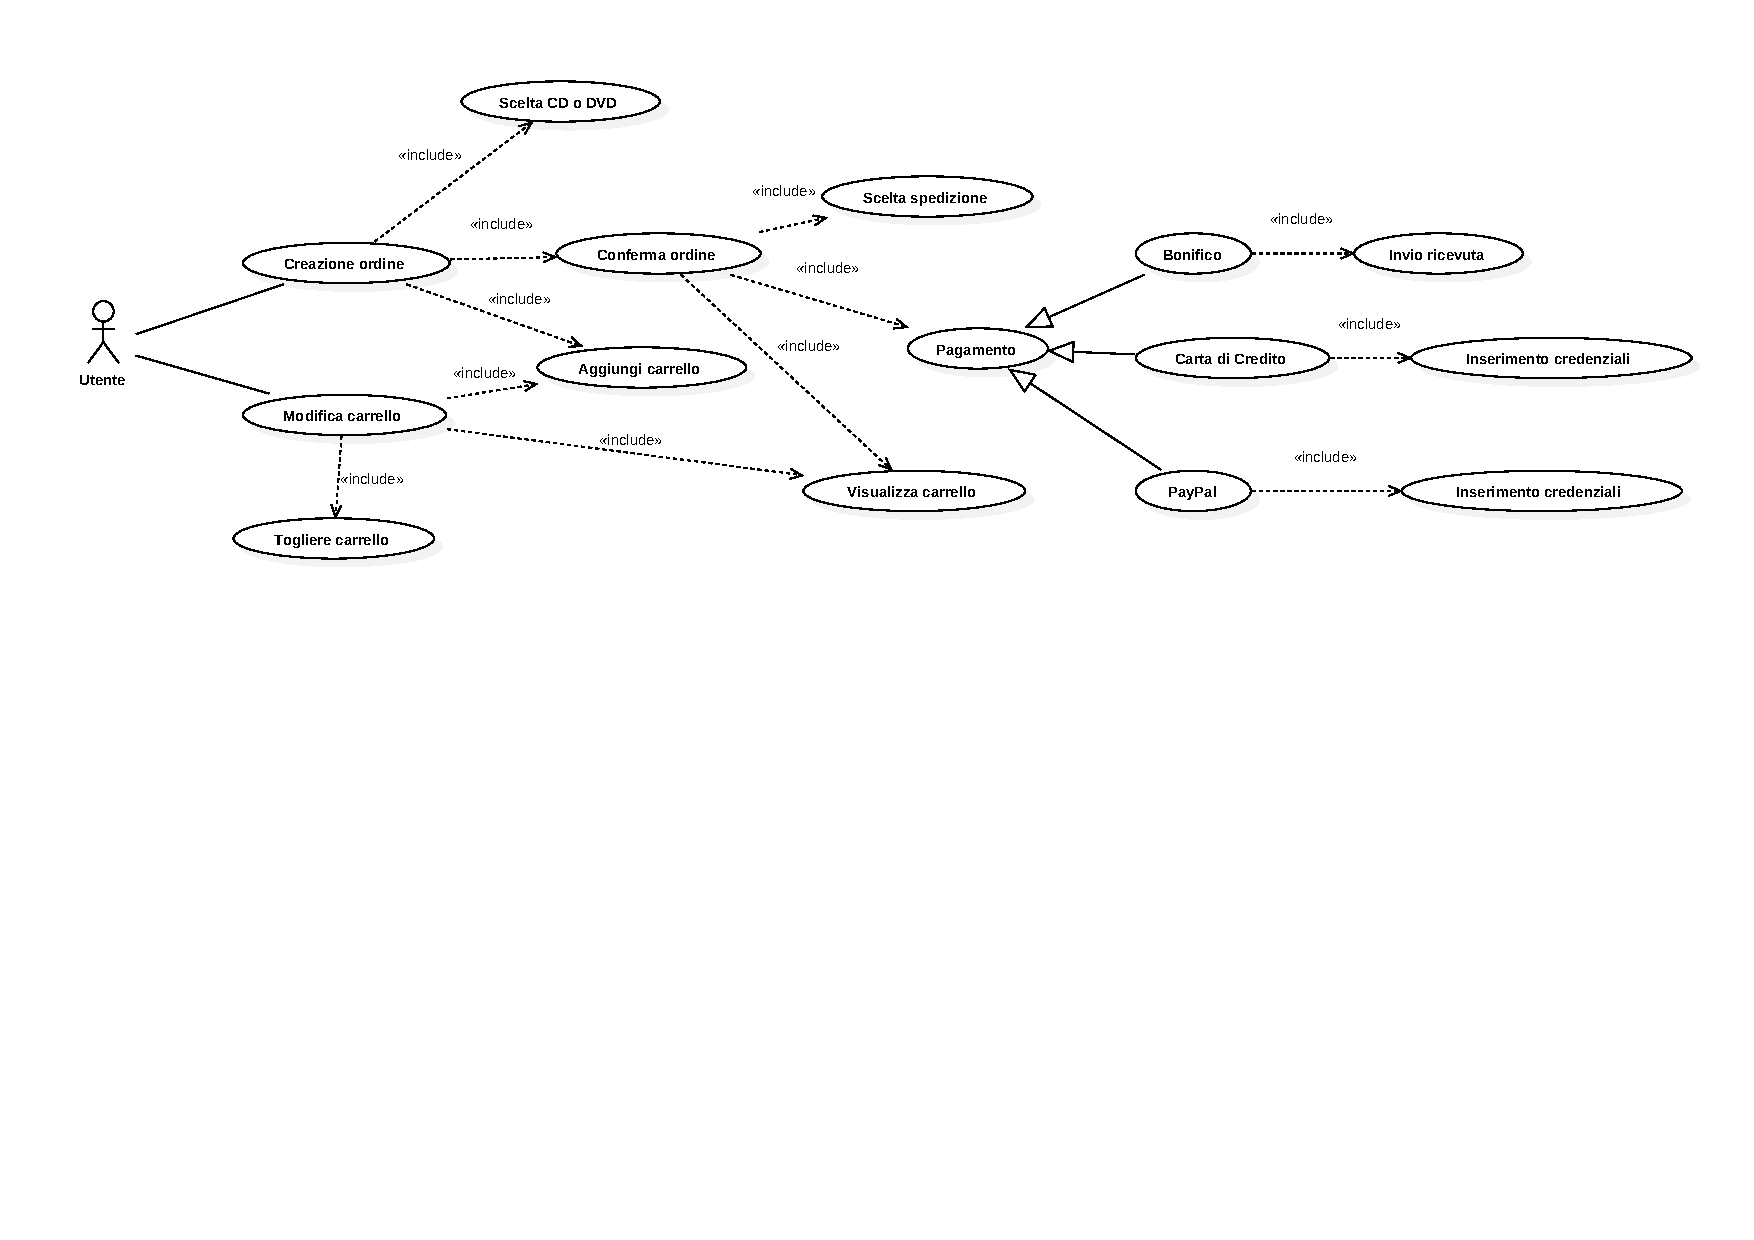
\includegraphics[width=350px]{img/Use2.pdf}
\caption{Use Case 2 \label{fig:use2}}
\end{figure}
\begin{figure}[H]
\center
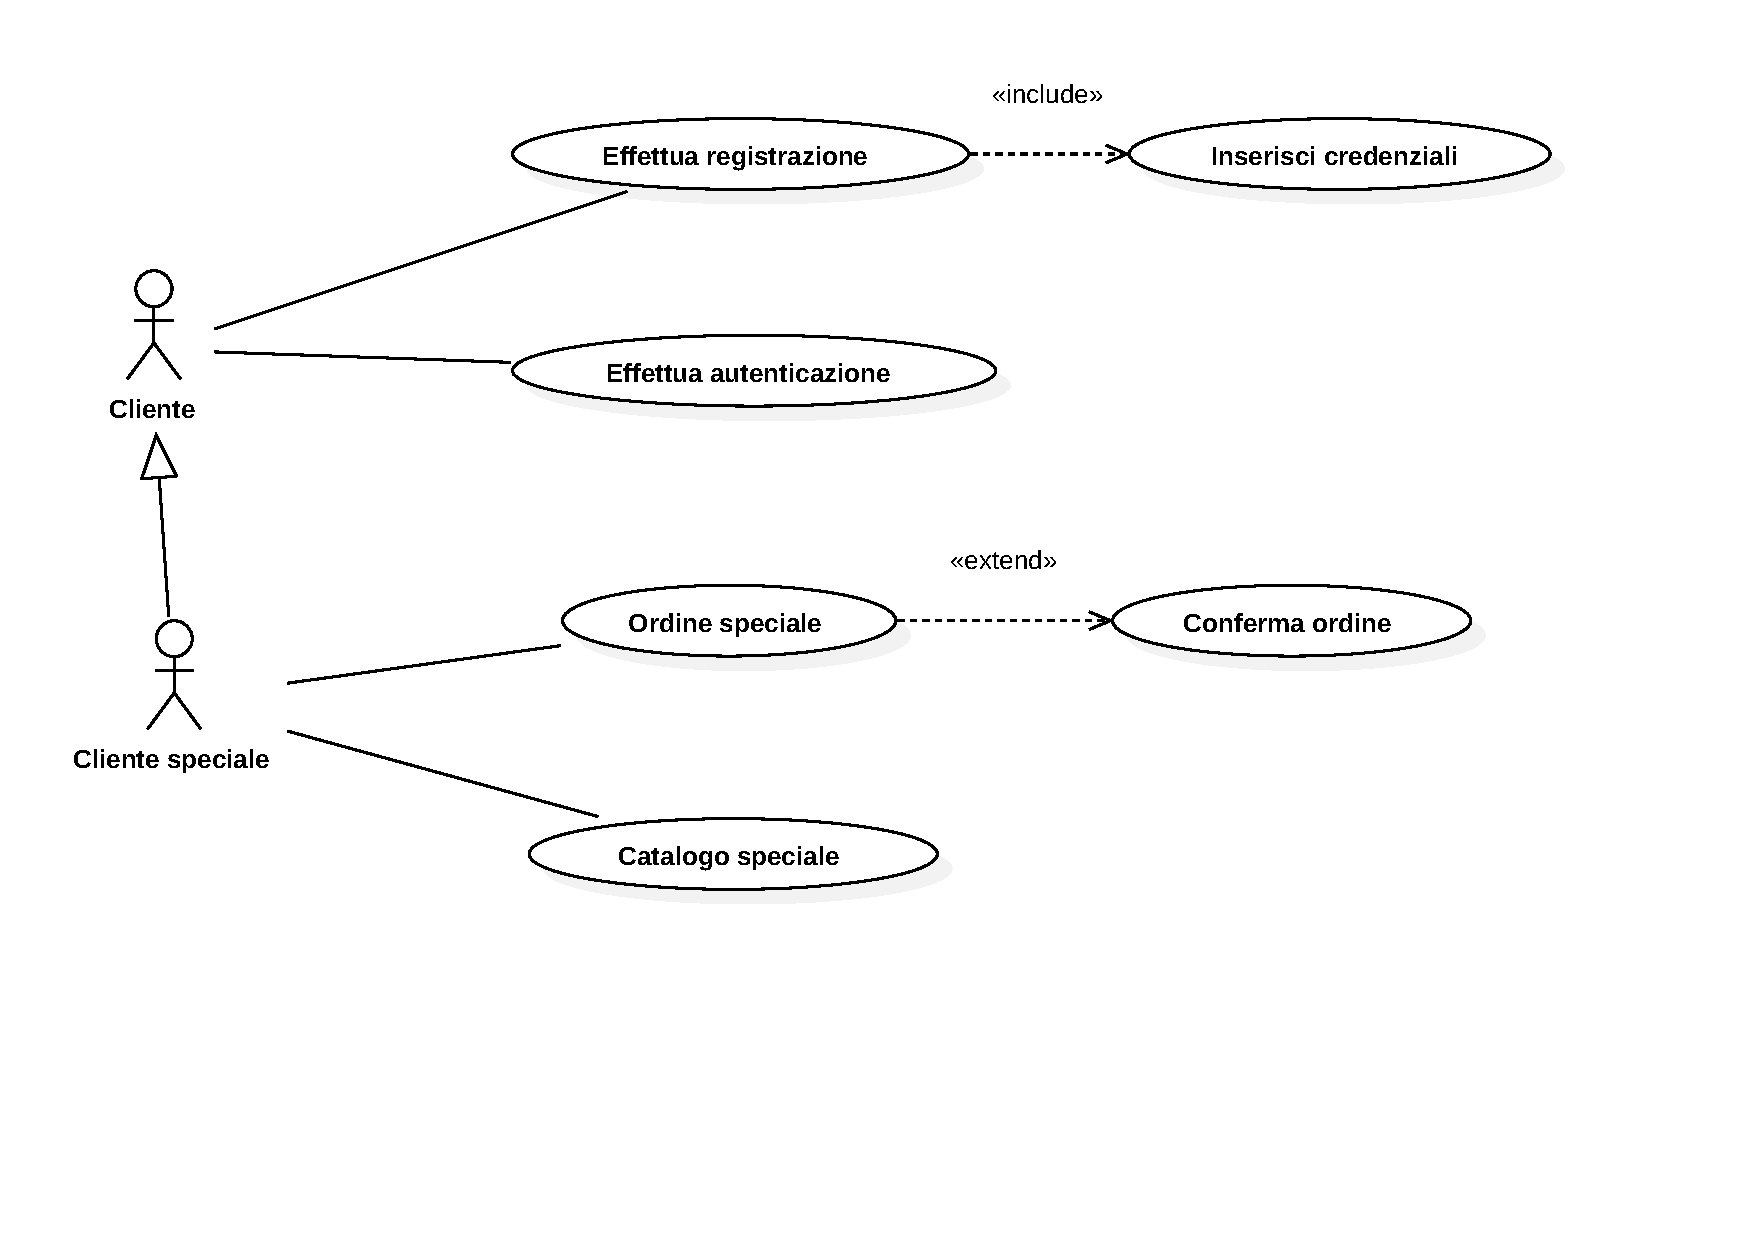
\includegraphics[width=350px]{img/Use3.pdf}
\caption{Use Case 3 \label{fig:use3}}
\end{figure}
\begin{figure}[H]
\center
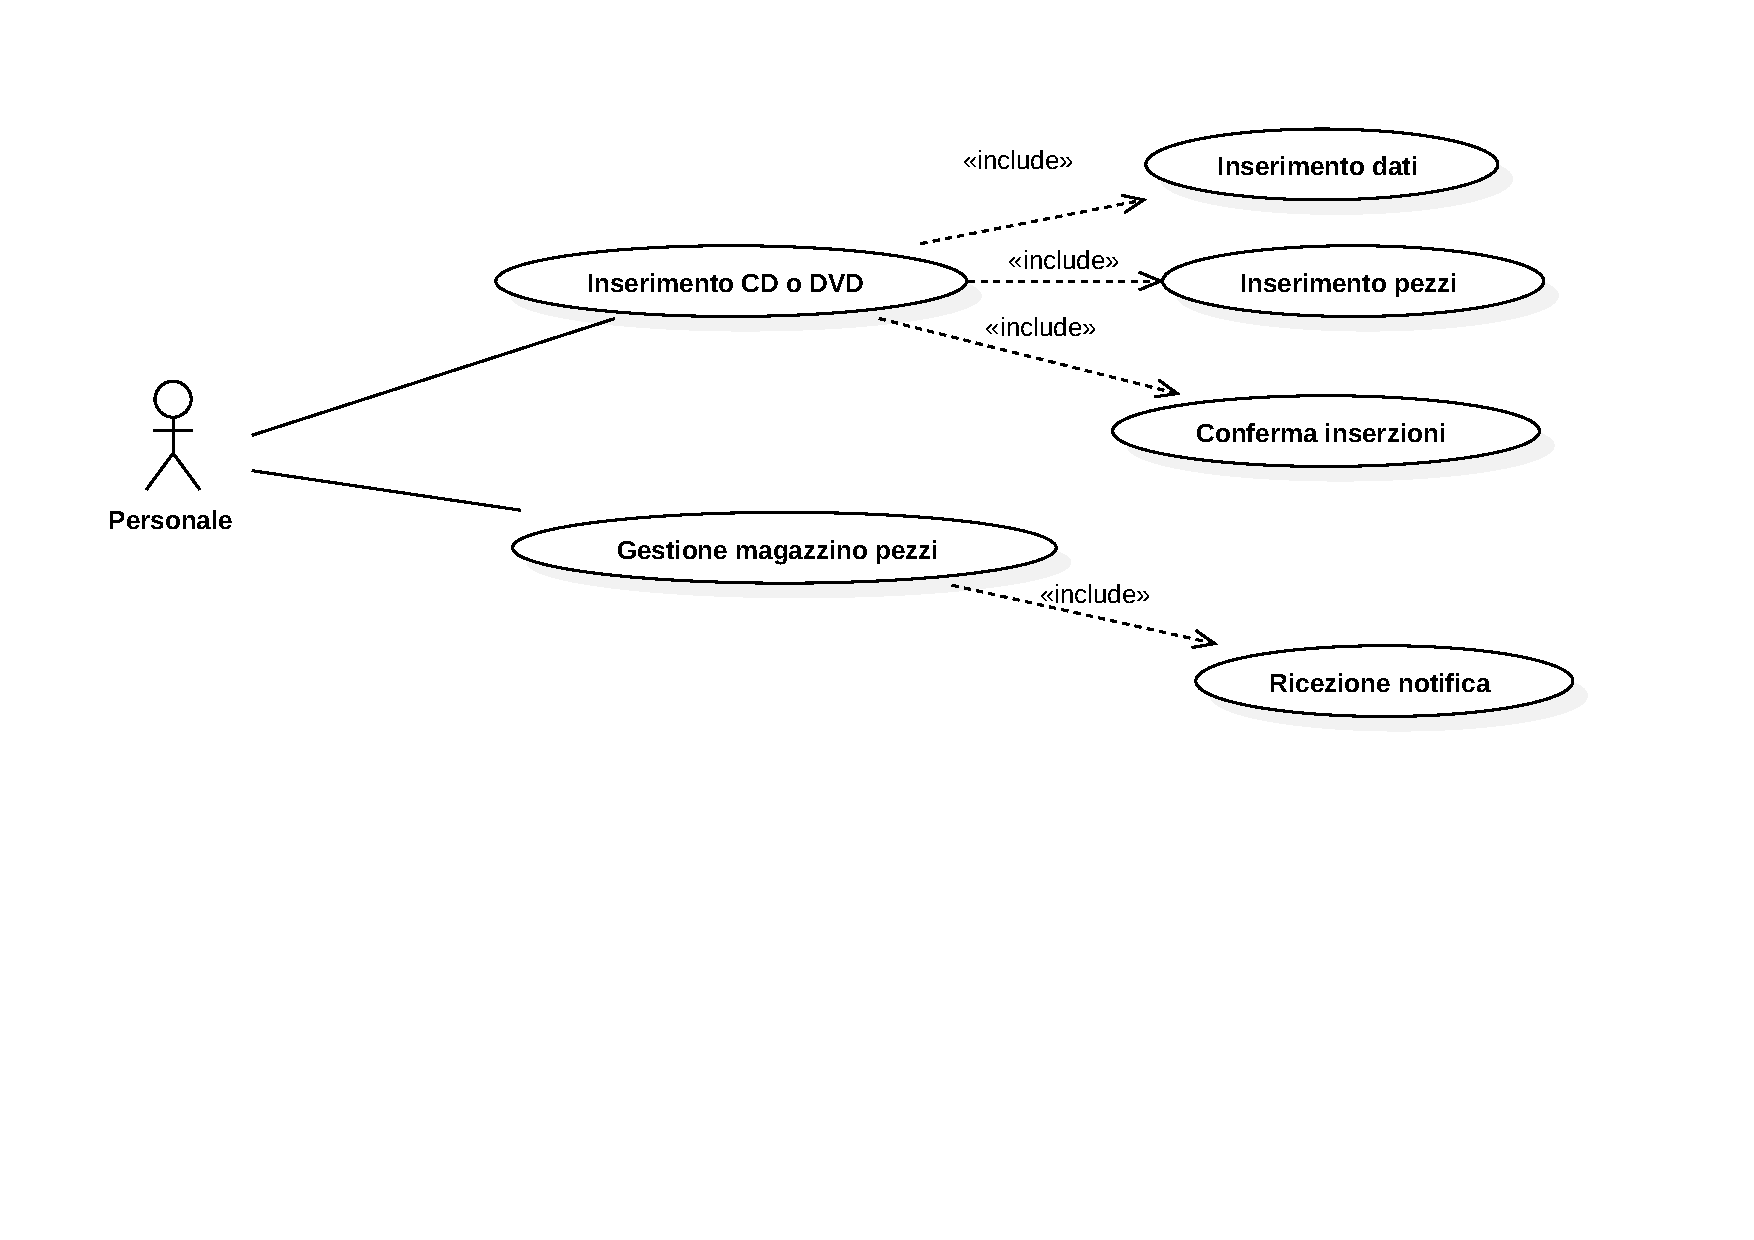
\includegraphics[width=350px]{img/Use4.pdf}
\caption{Use Case 4 \label{fig:use4}}
\end{figure}

\section{Sequence Diagram}
\begin{figure}[H]
\center
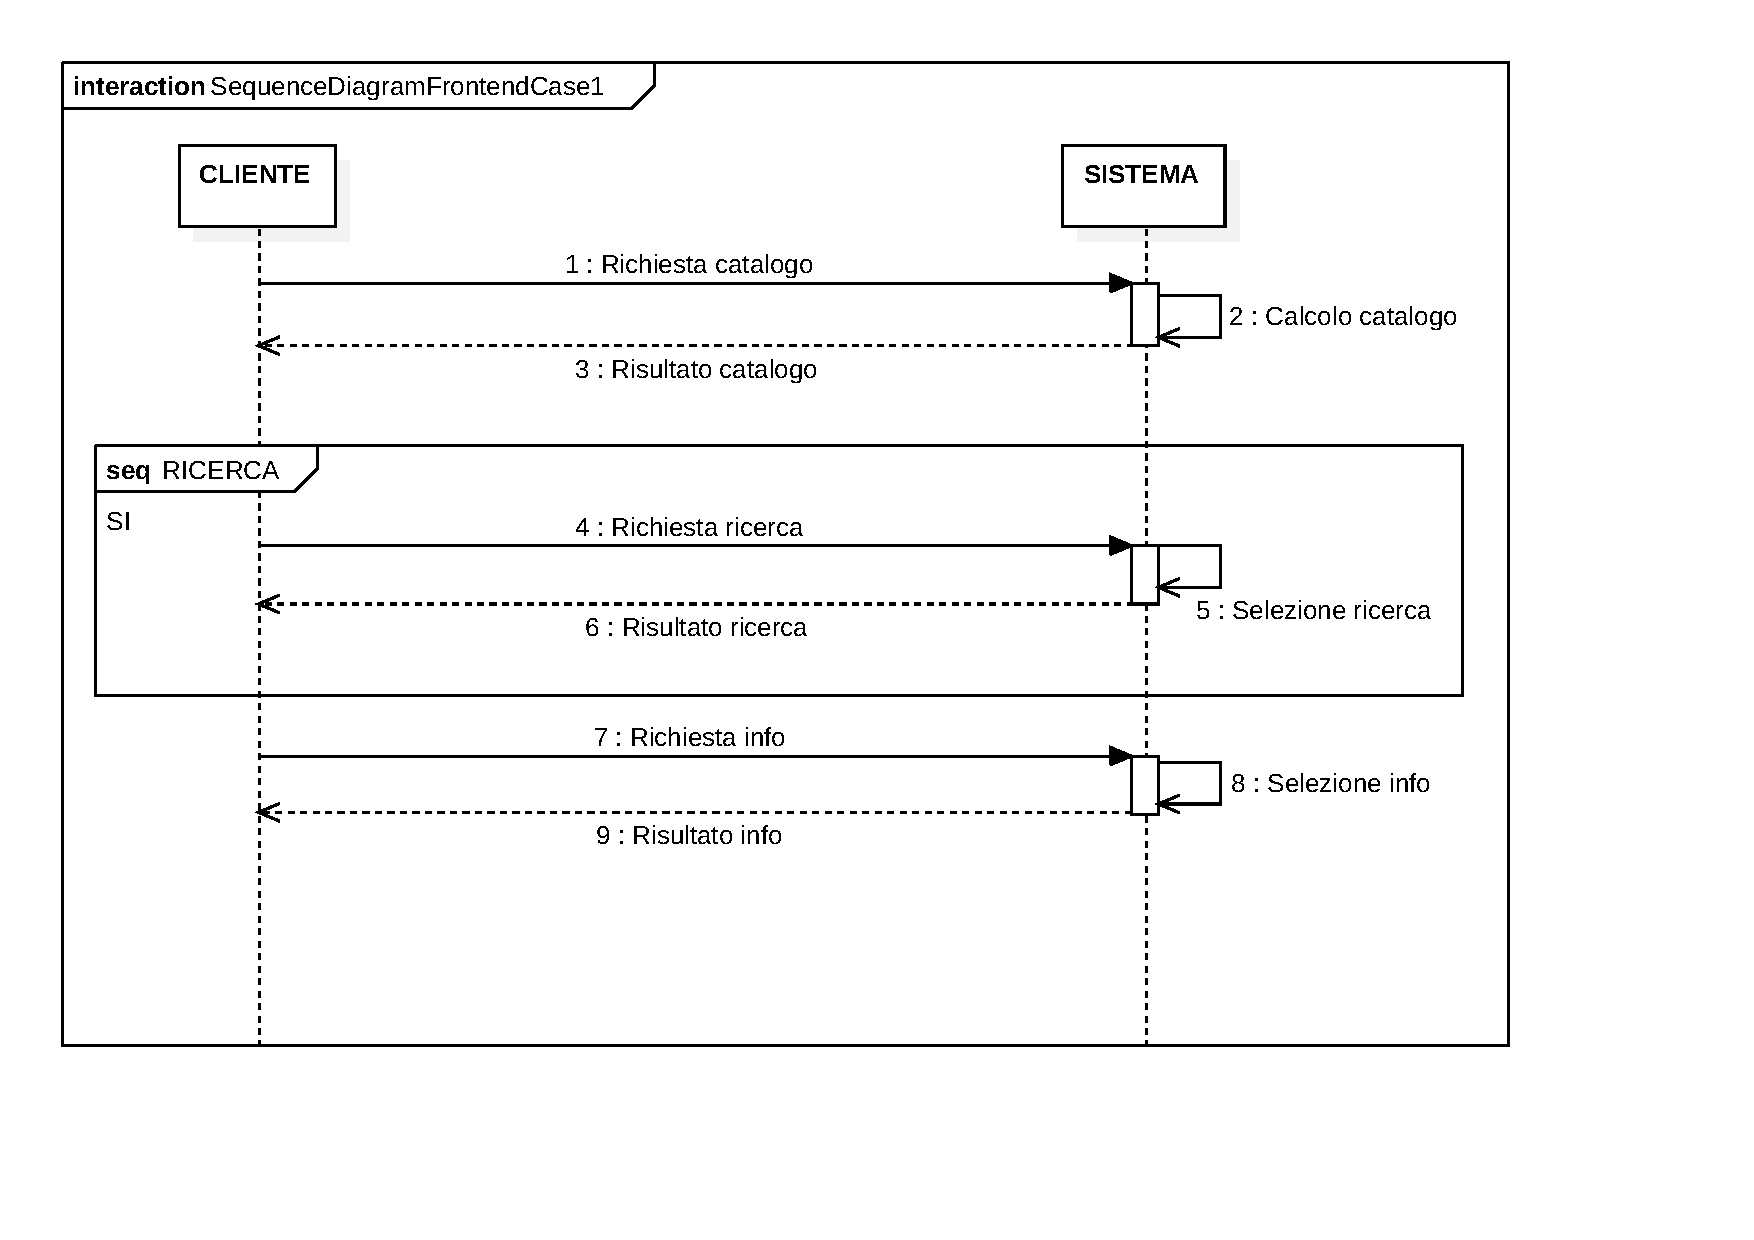
\includegraphics[width=350px]{img/Seq1F.pdf}
\caption{Diagramma di sequenza 1 front-end \label{fig:seq1f}}
\end{figure}
\begin{figure}[H]
\center
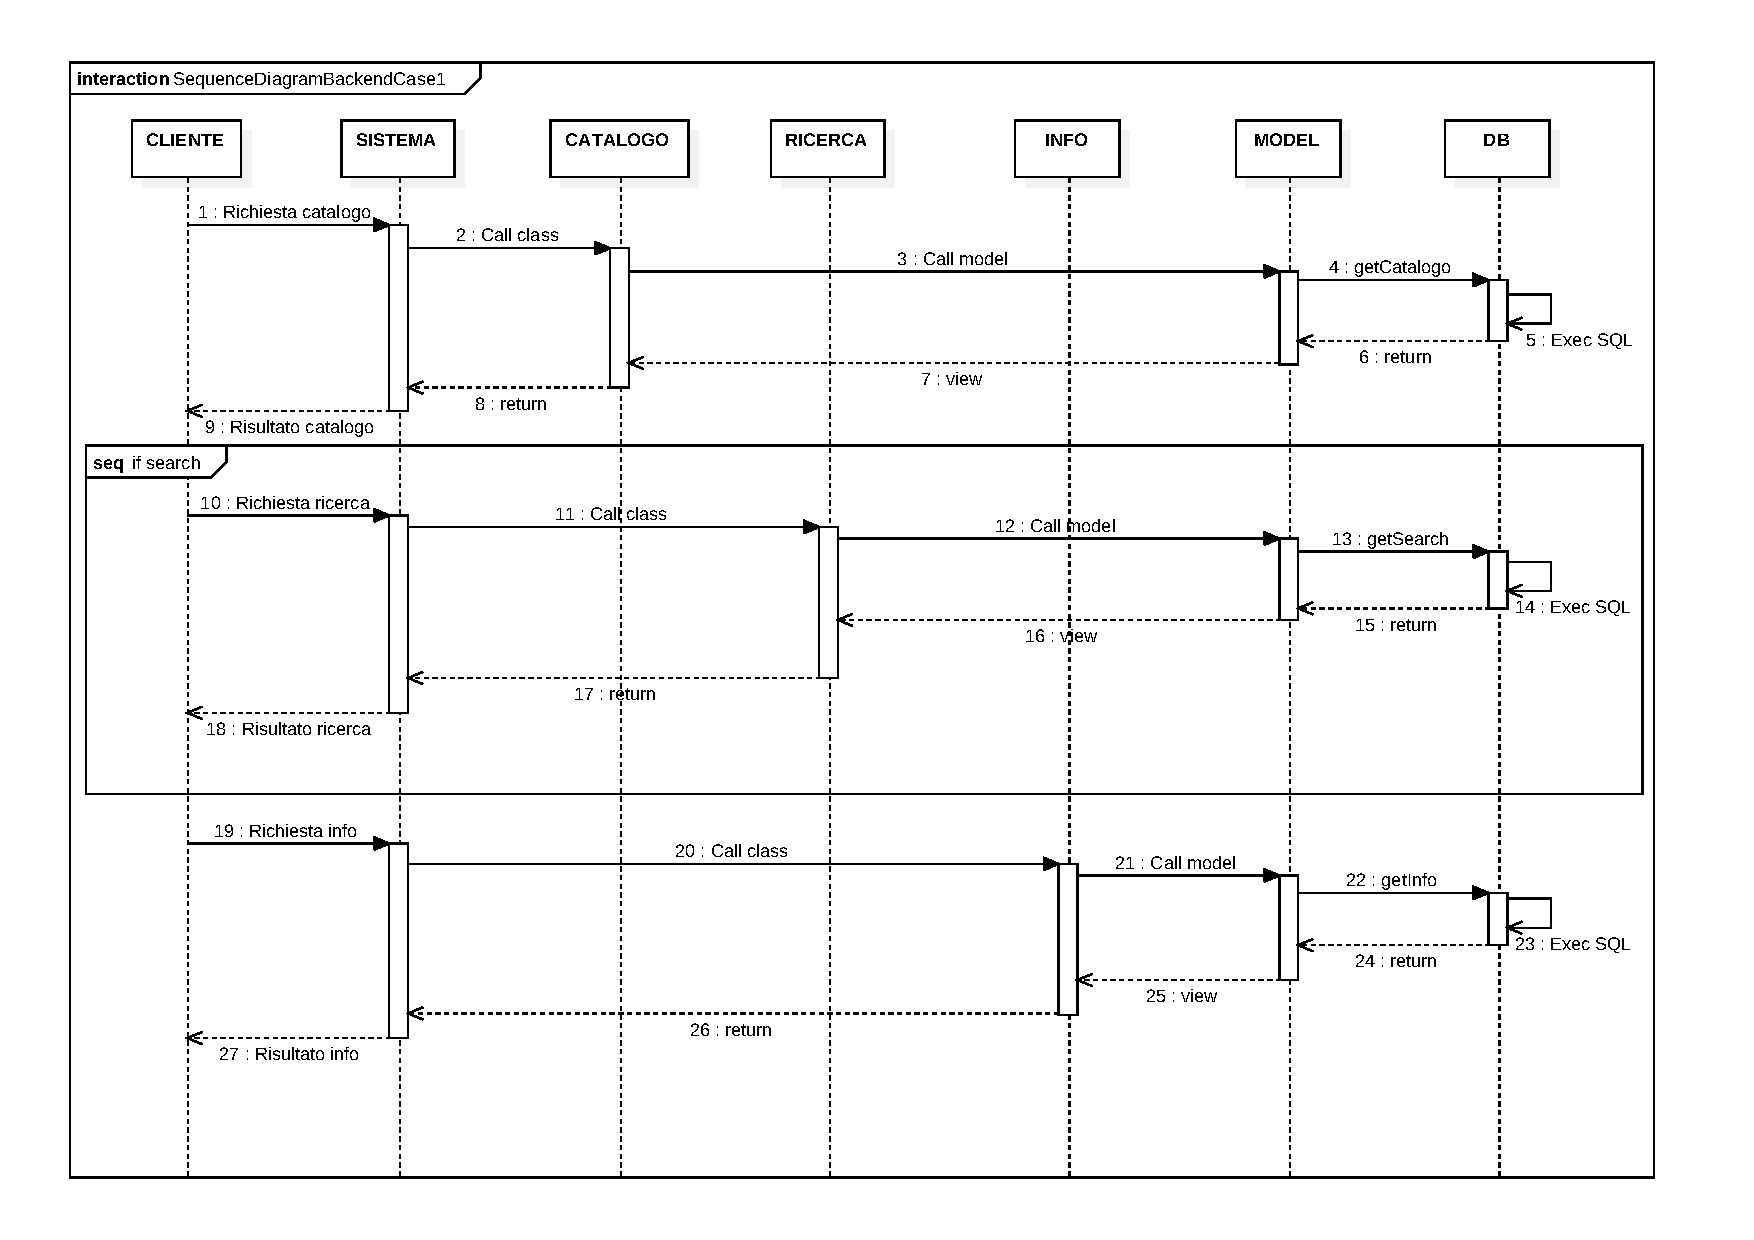
\includegraphics[width=350px]{img/Seq1B.pdf}
\caption{Diagramma di sequenza 1 back-end \label{fig:seq1b}}
\end{figure}
\begin{figure}[H]
\center
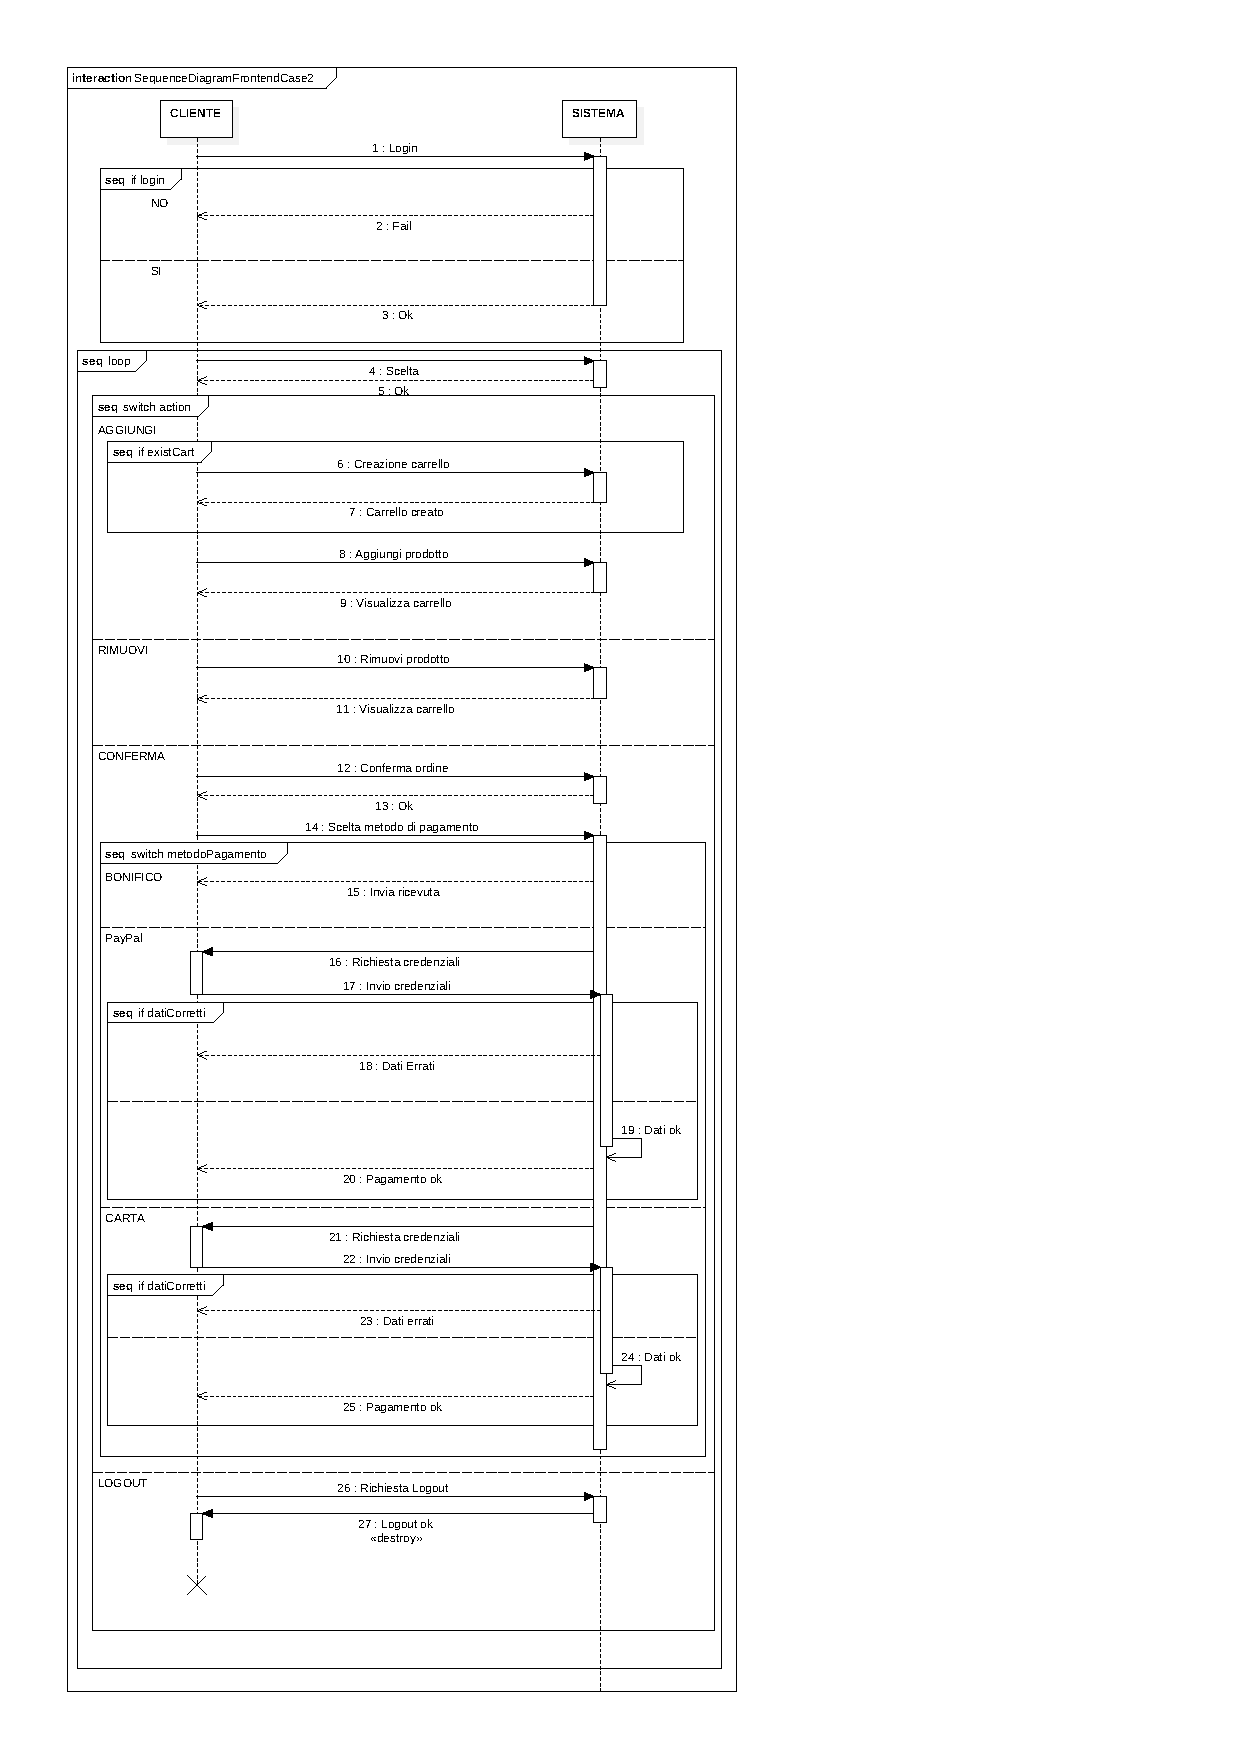
\includegraphics[width=225px]{img/Seq2F.pdf}
\caption{Diagramma di sequenza 2 front-end \label{fig:seq2f}}
\end{figure}
\begin{figure}[H]
\center
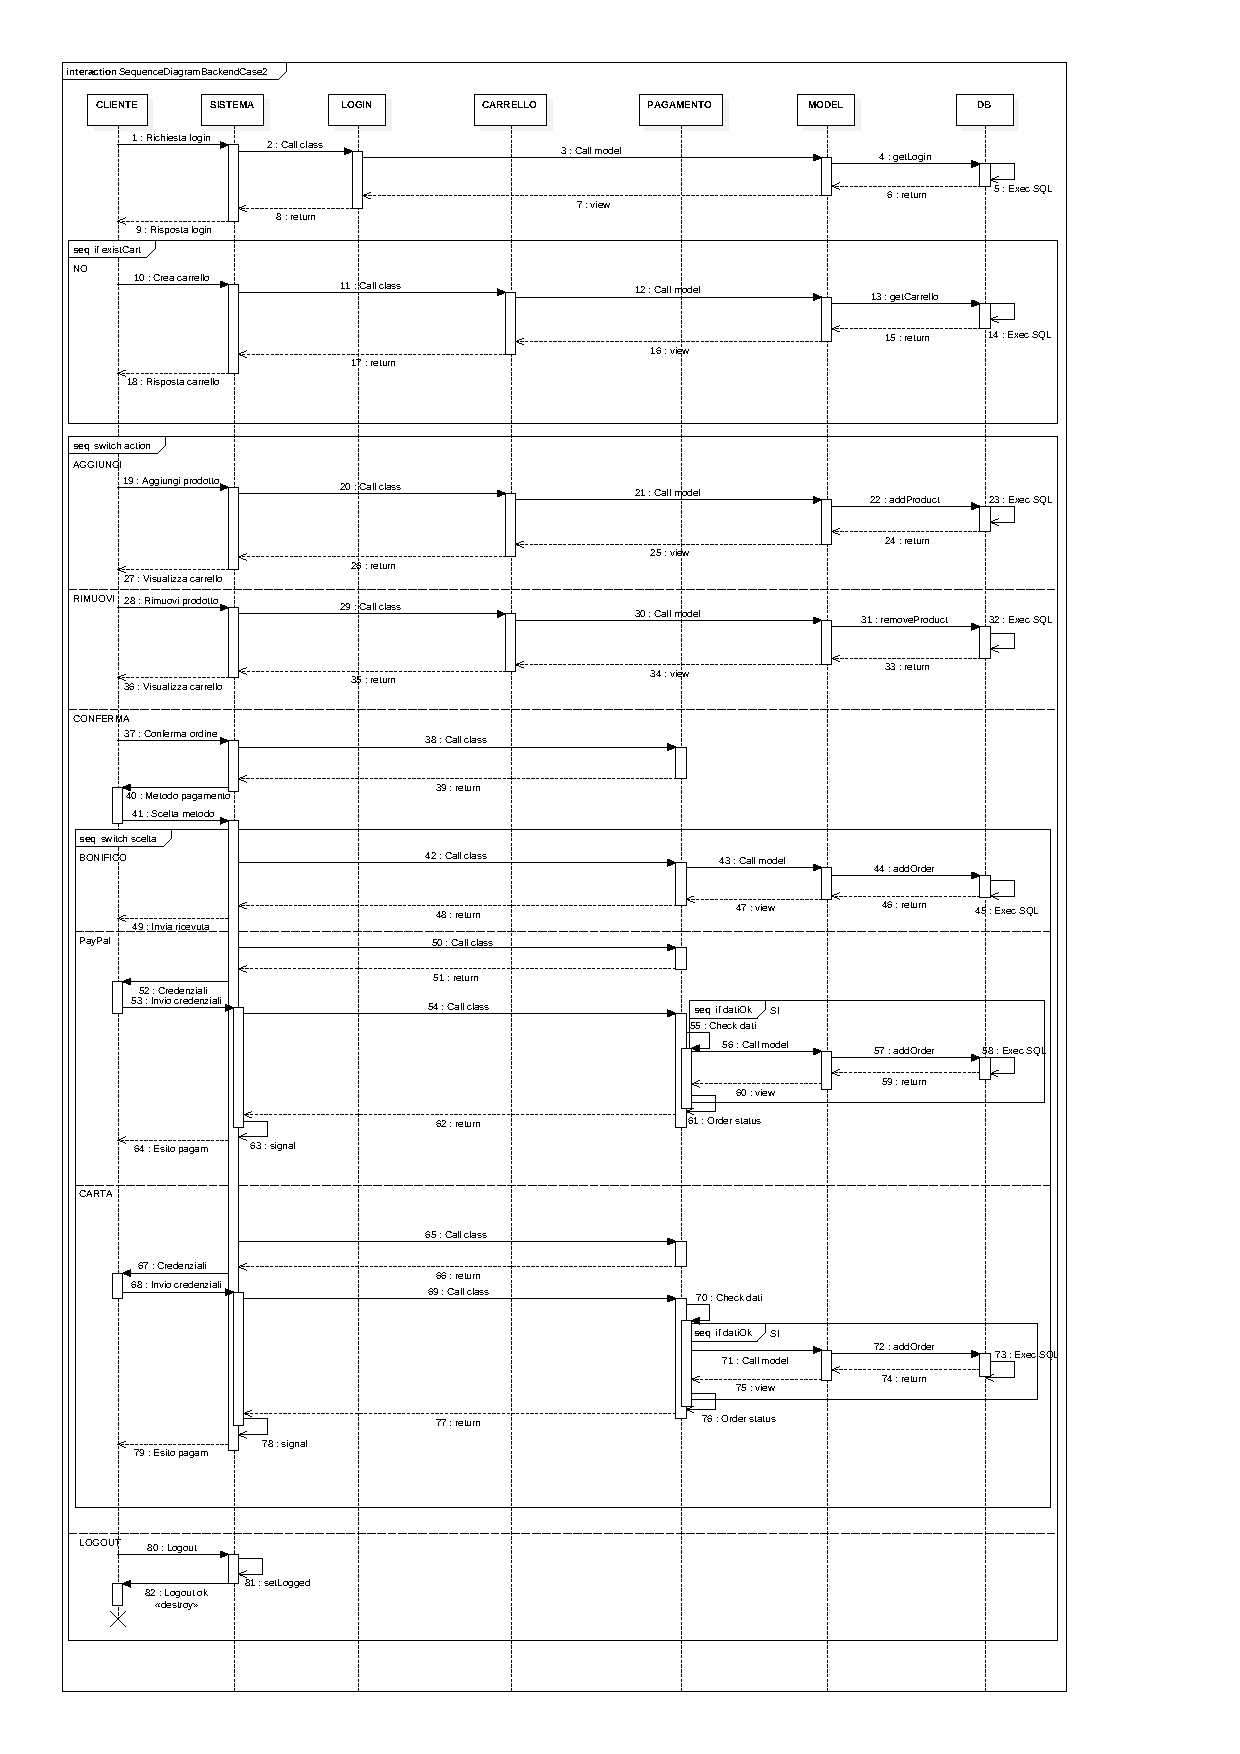
\includegraphics[width=350px]{img/Seq2B.pdf}
\caption{Diagramma di sequenza 2 back-end \label{fig:seq2b}}
\end{figure}
\begin{figure}[H]
\center
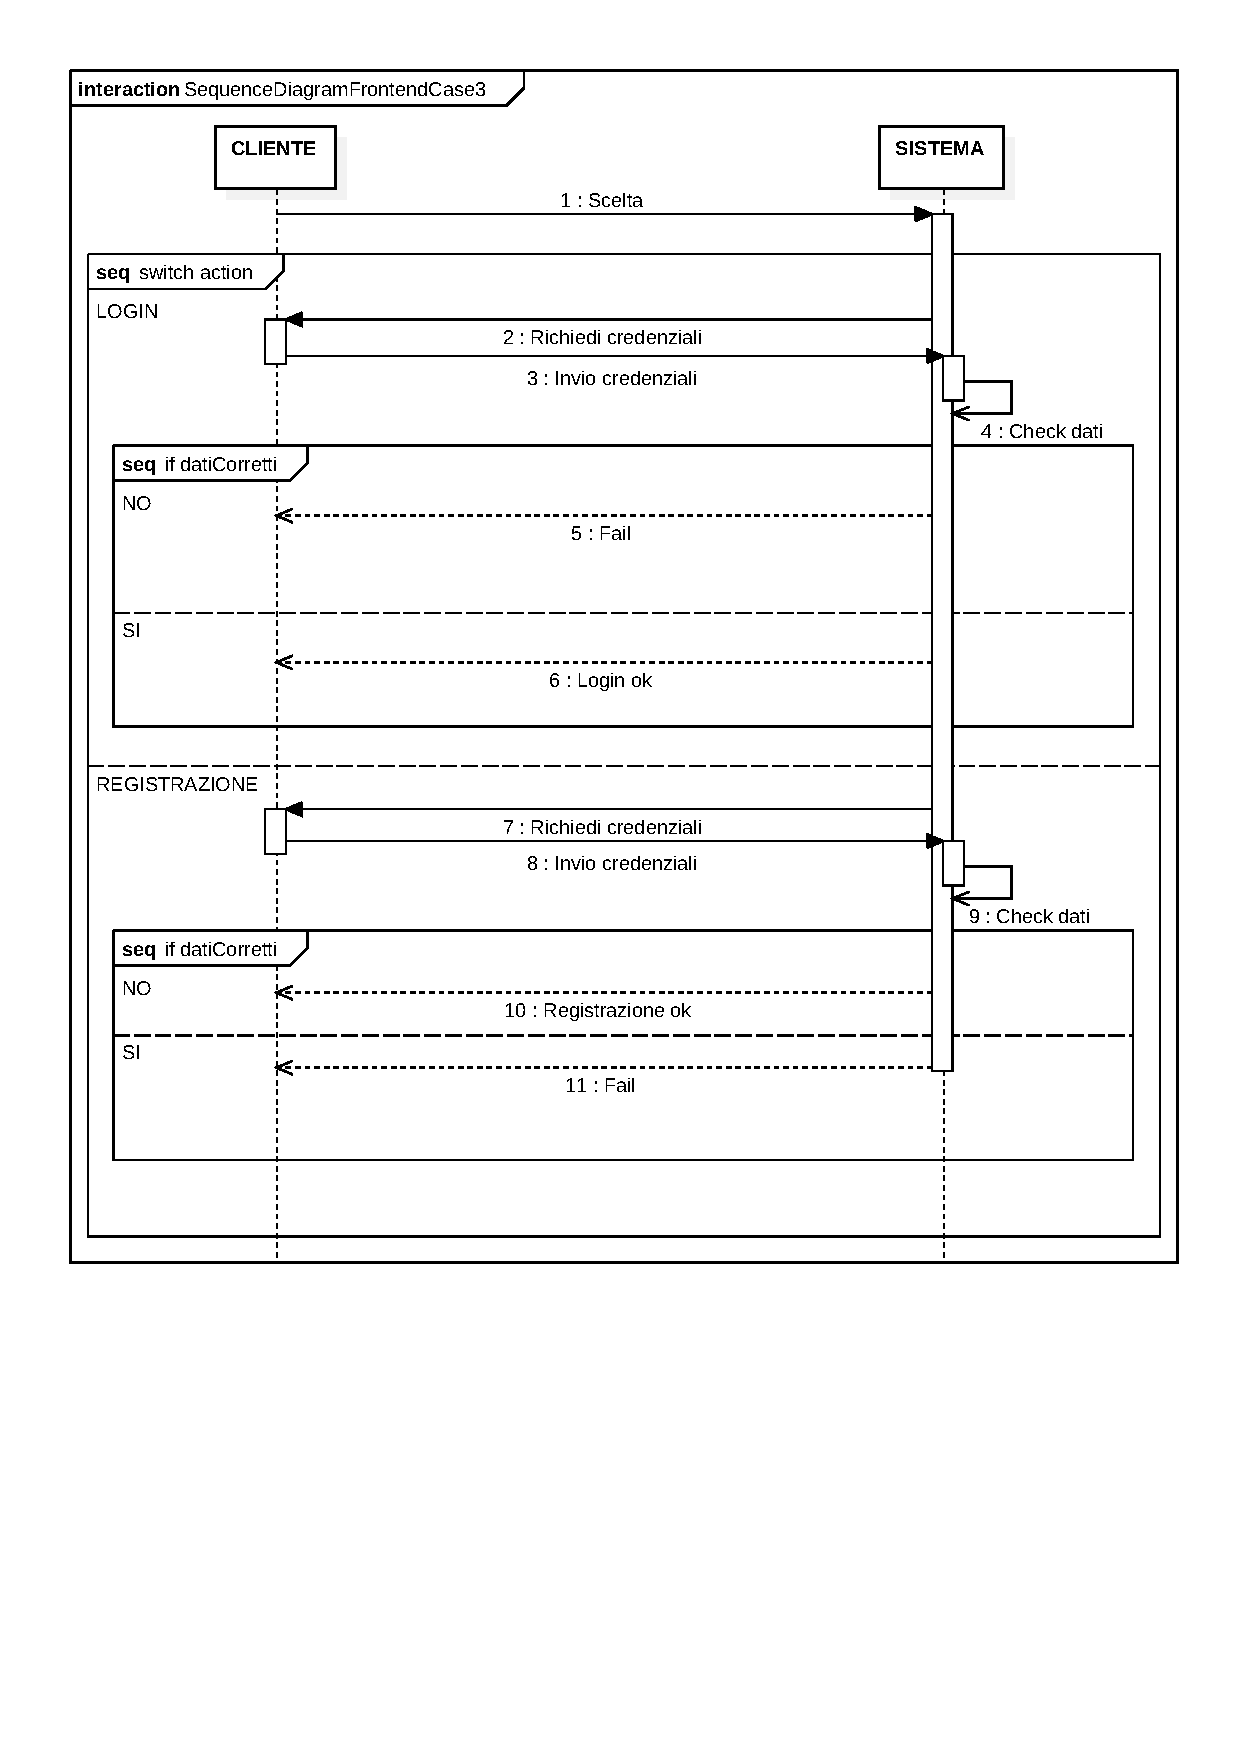
\includegraphics[width=225px]{img/Seq3F.pdf}
\caption{Diagramma di sequenza 3 front-end \label{fig:seq3f}}
\end{figure}
\begin{figure}[H]
\center
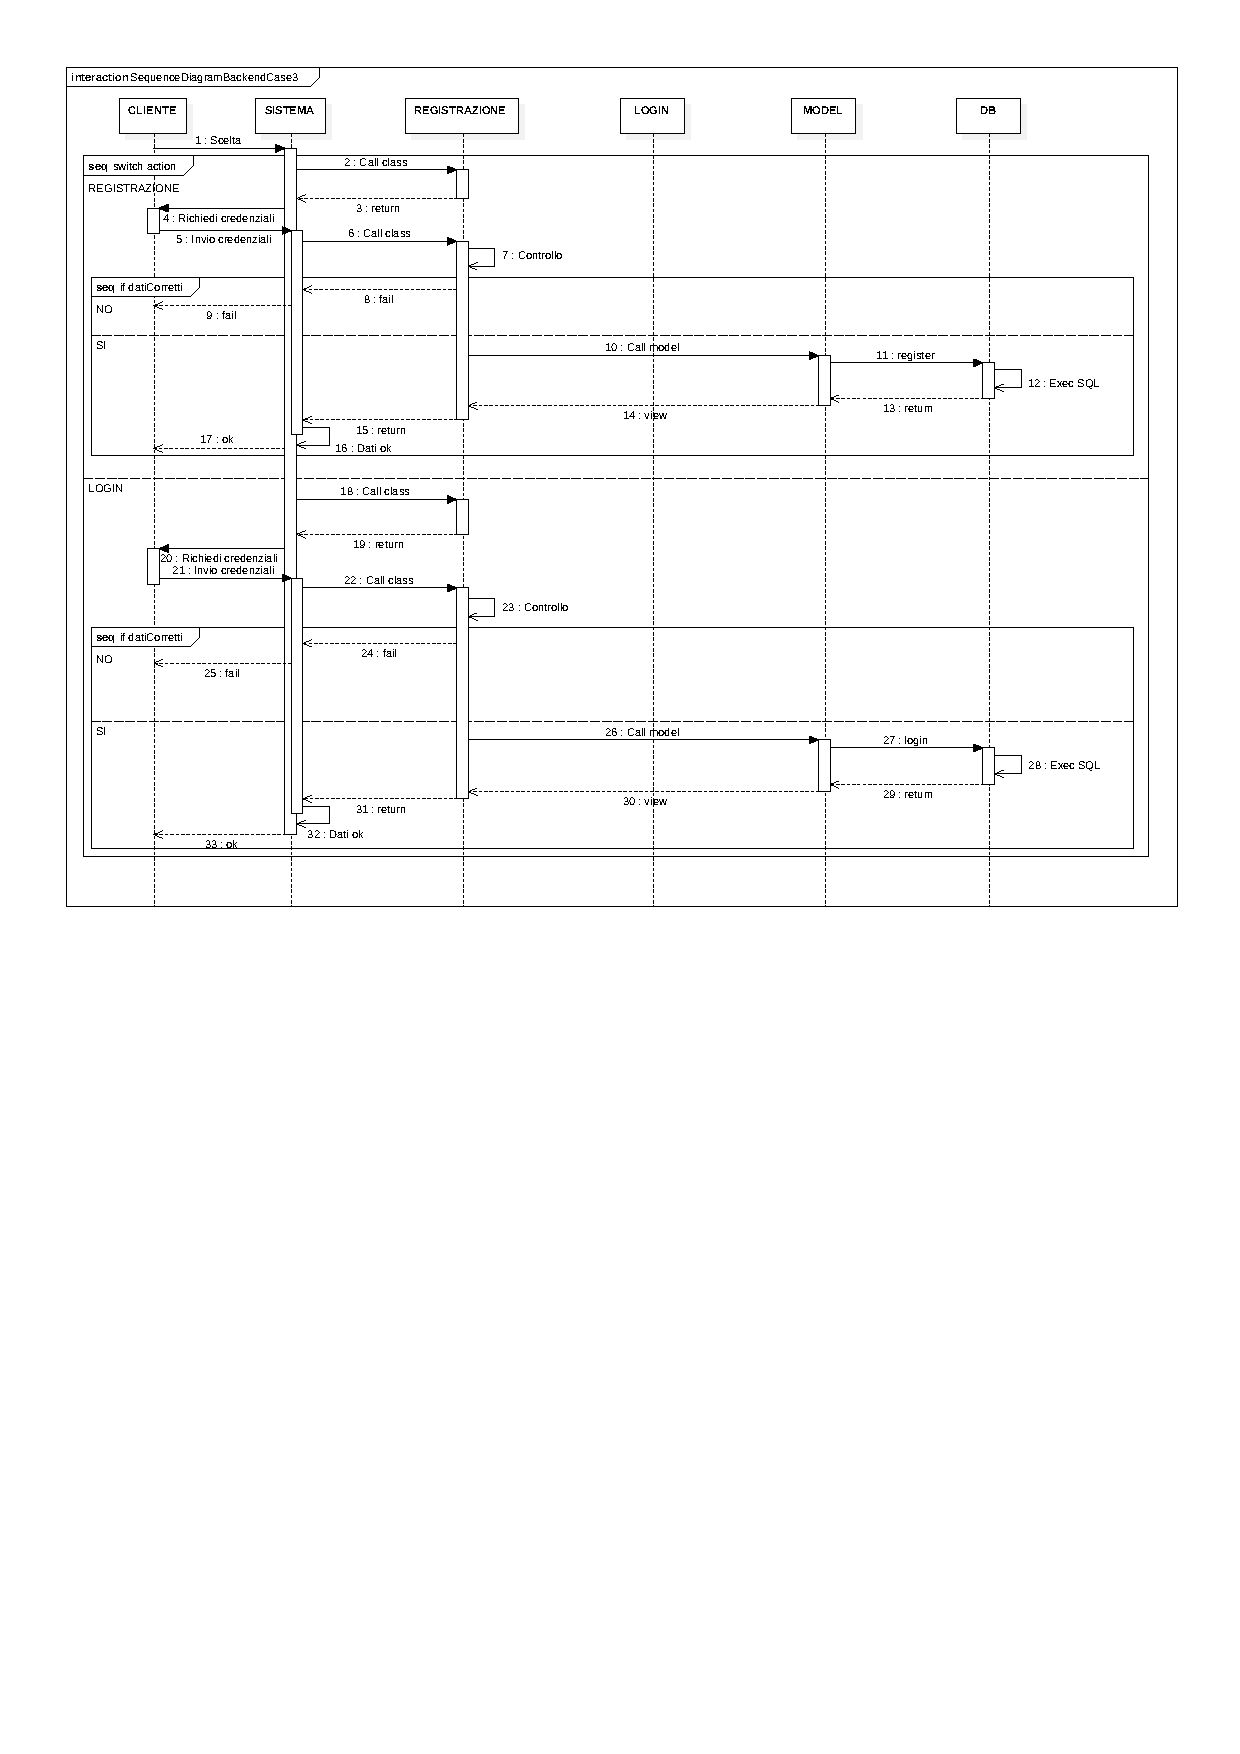
\includegraphics[width=350px]{img/Seq3B.pdf}
\caption{Diagramma di sequenza 3 back-end \label{fig:seq3b}}
\end{figure}
\begin{figure}[H]
\center
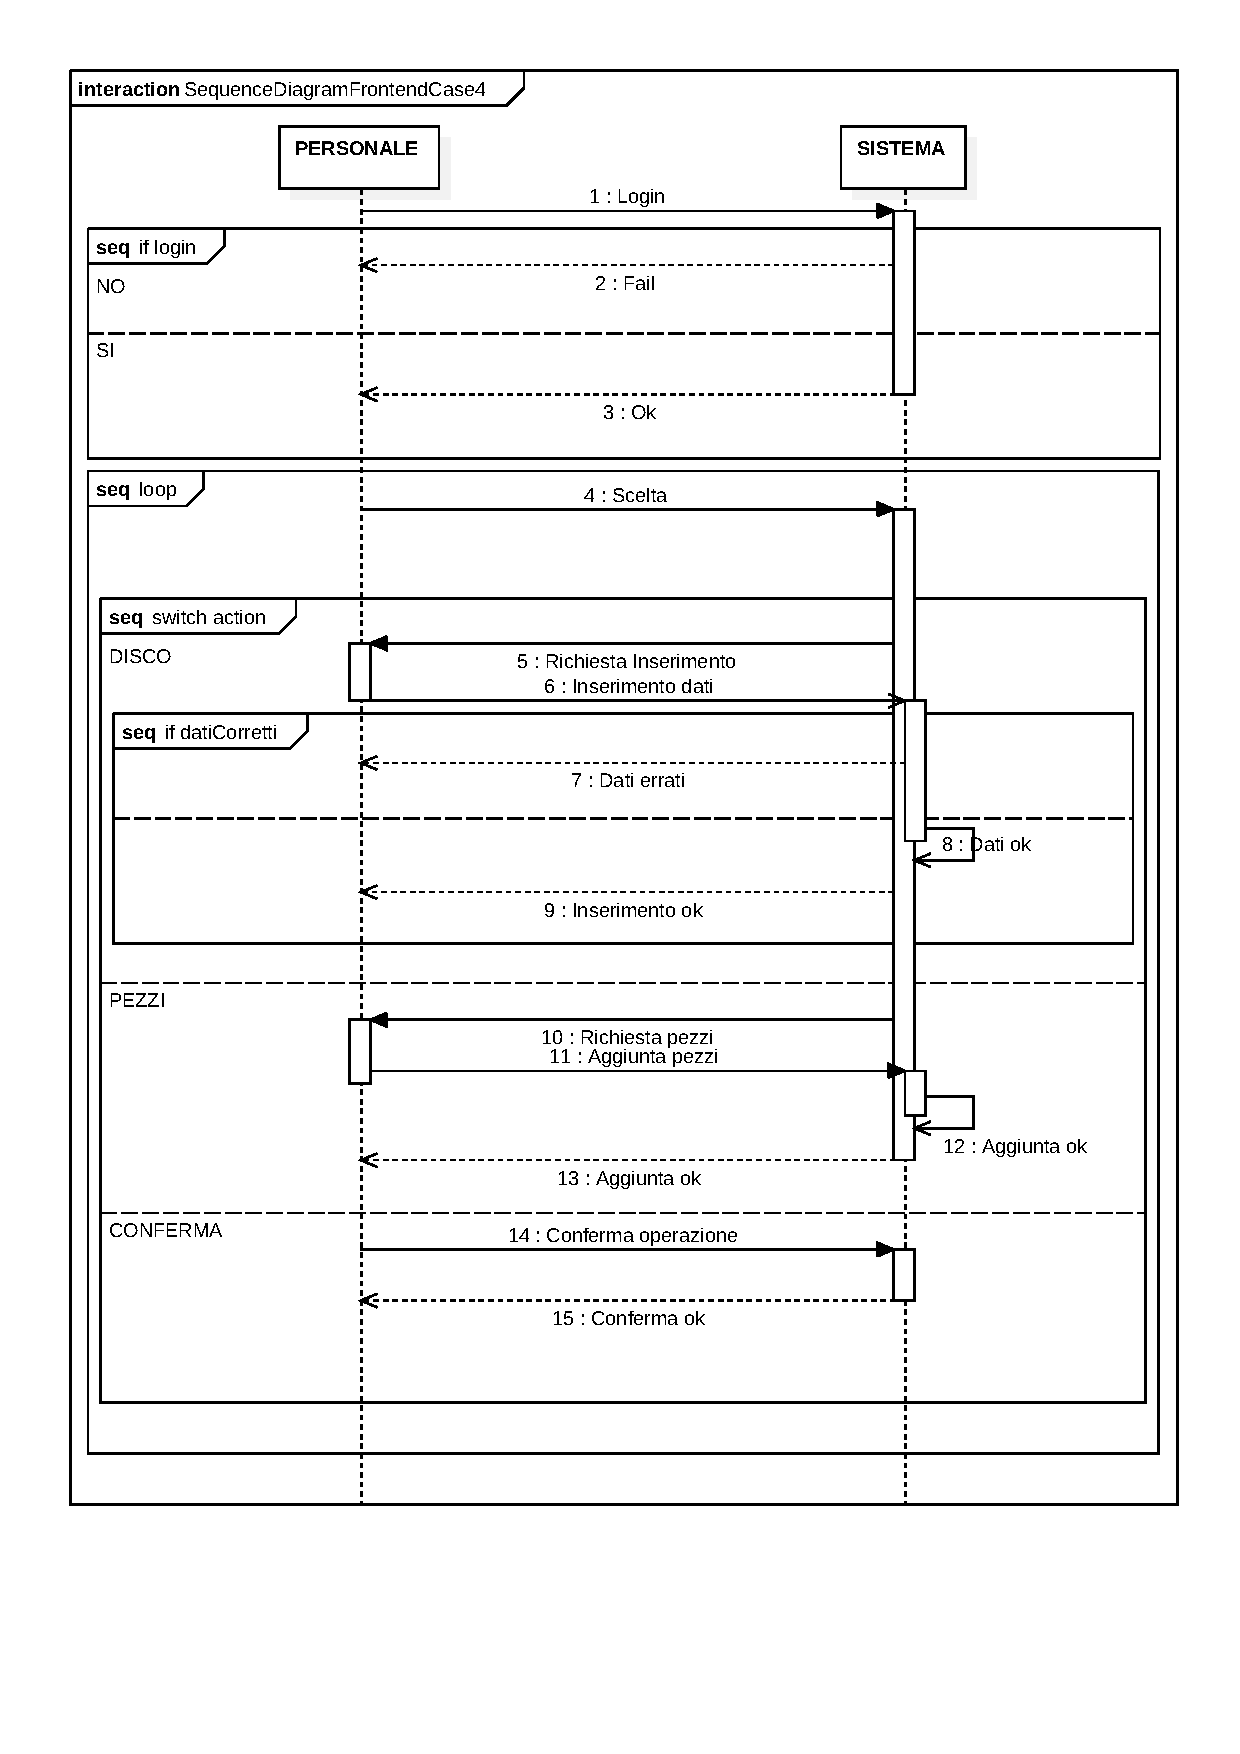
\includegraphics[width=225px]{img/Seq4F1.pdf}
\caption{Diagramma di sequenza 4 front-end 1 \label{fig:seq4f1}}
\end{figure}
\begin{figure}[H]
\center
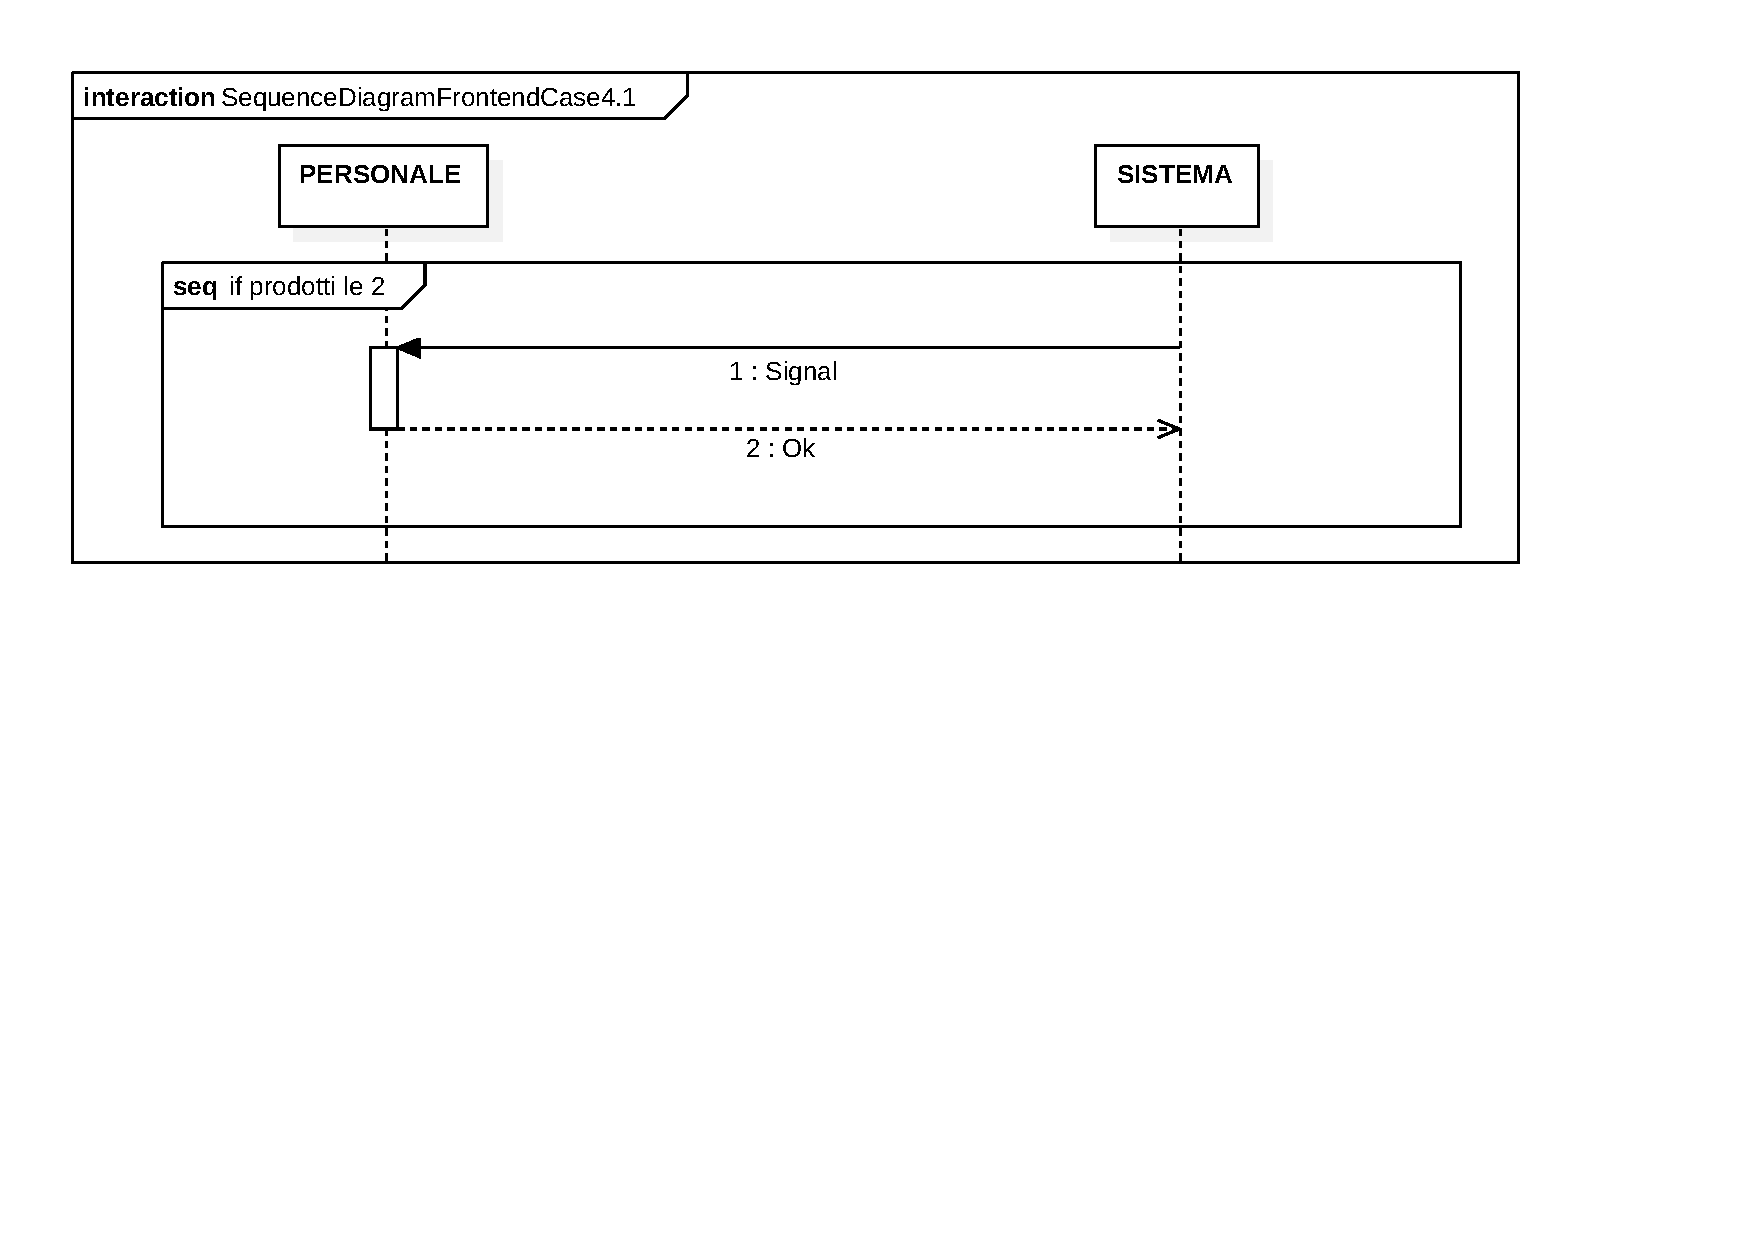
\includegraphics[width=350px]{img/Seq4F2.pdf}
\caption{Diagramma di sequenza 4 front-end  2\label{fig:seq4f2}}
\end{figure}


\section{Activity Diagram}
\begin{figure}[H]
\center
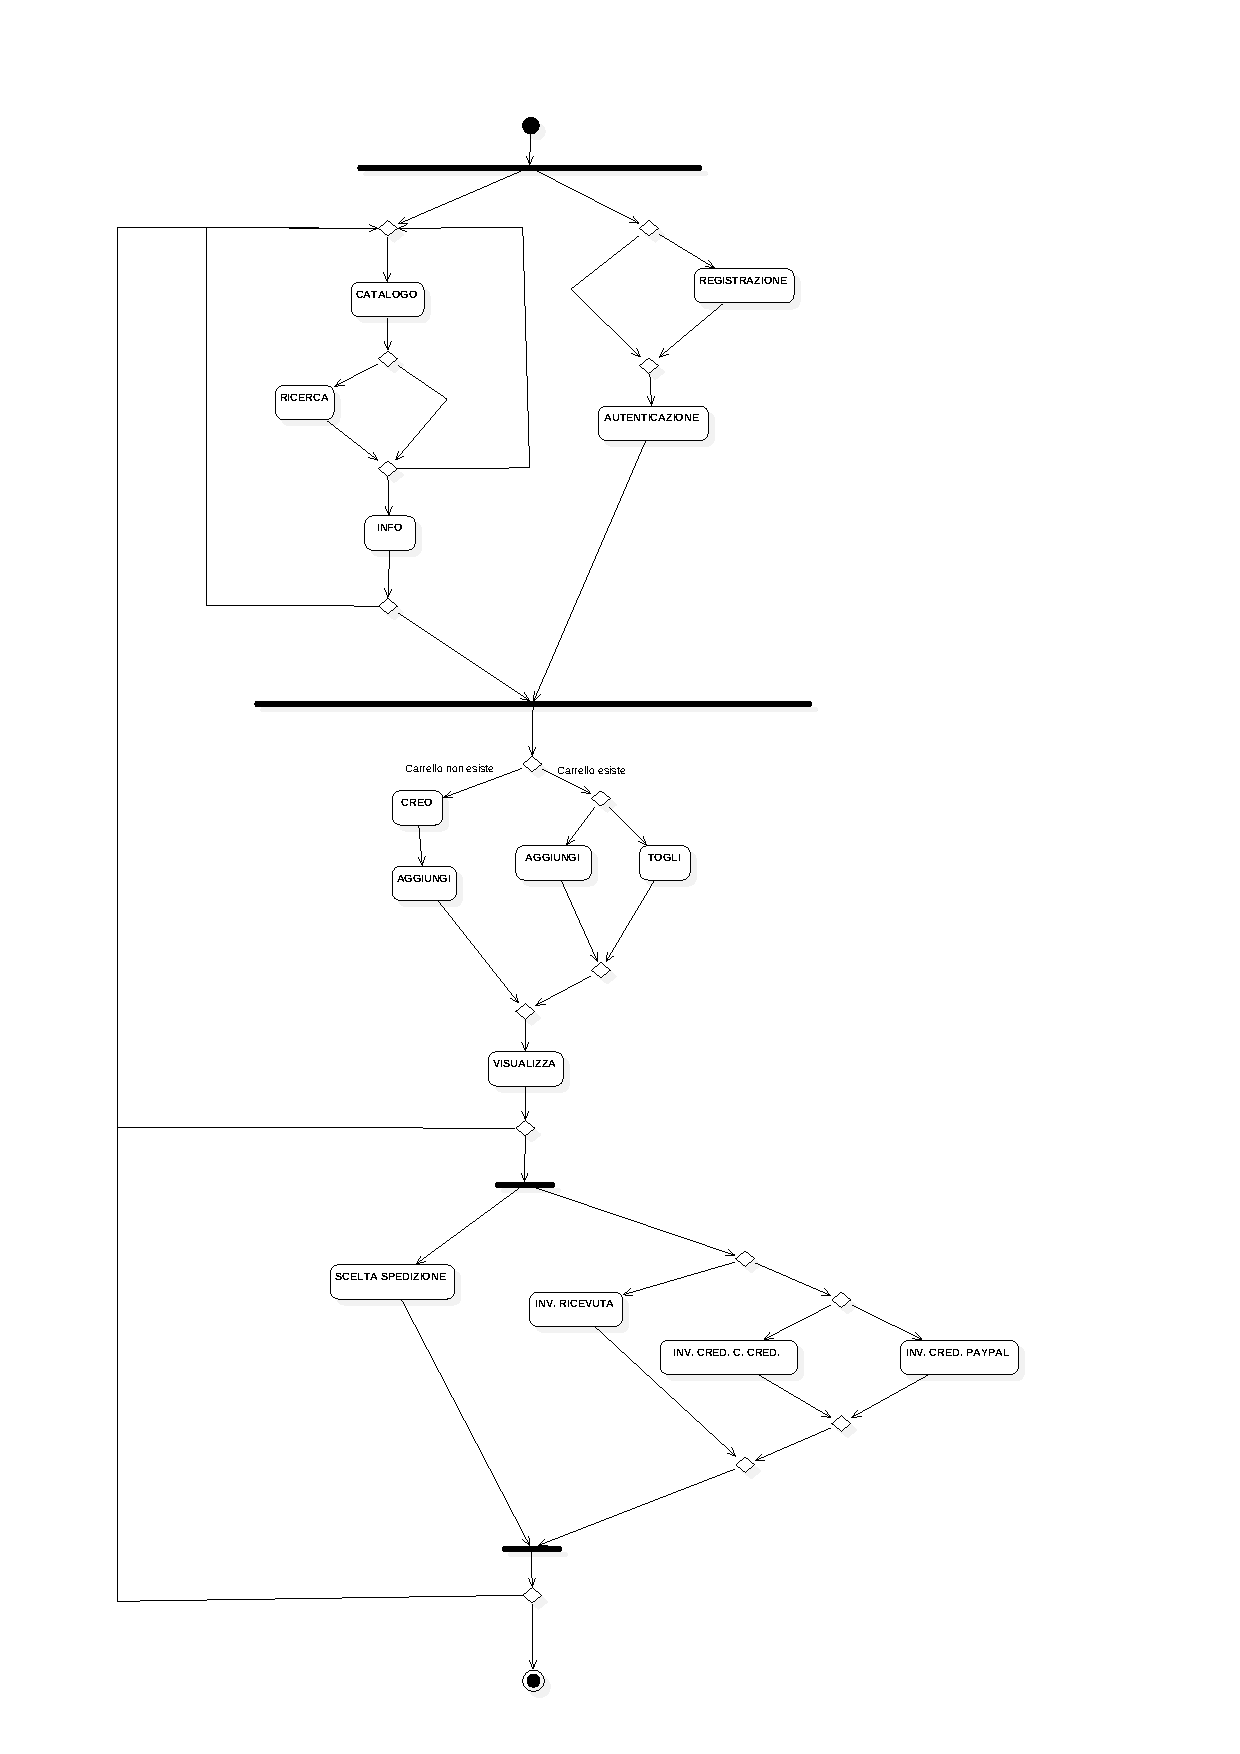
\includegraphics[width=350px]{img/Activity.pdf}
\caption{Activity Diagram \label{fig:act}}
\end{figure}

\section{Class Diagram}
\begin{figure}[H]
\center
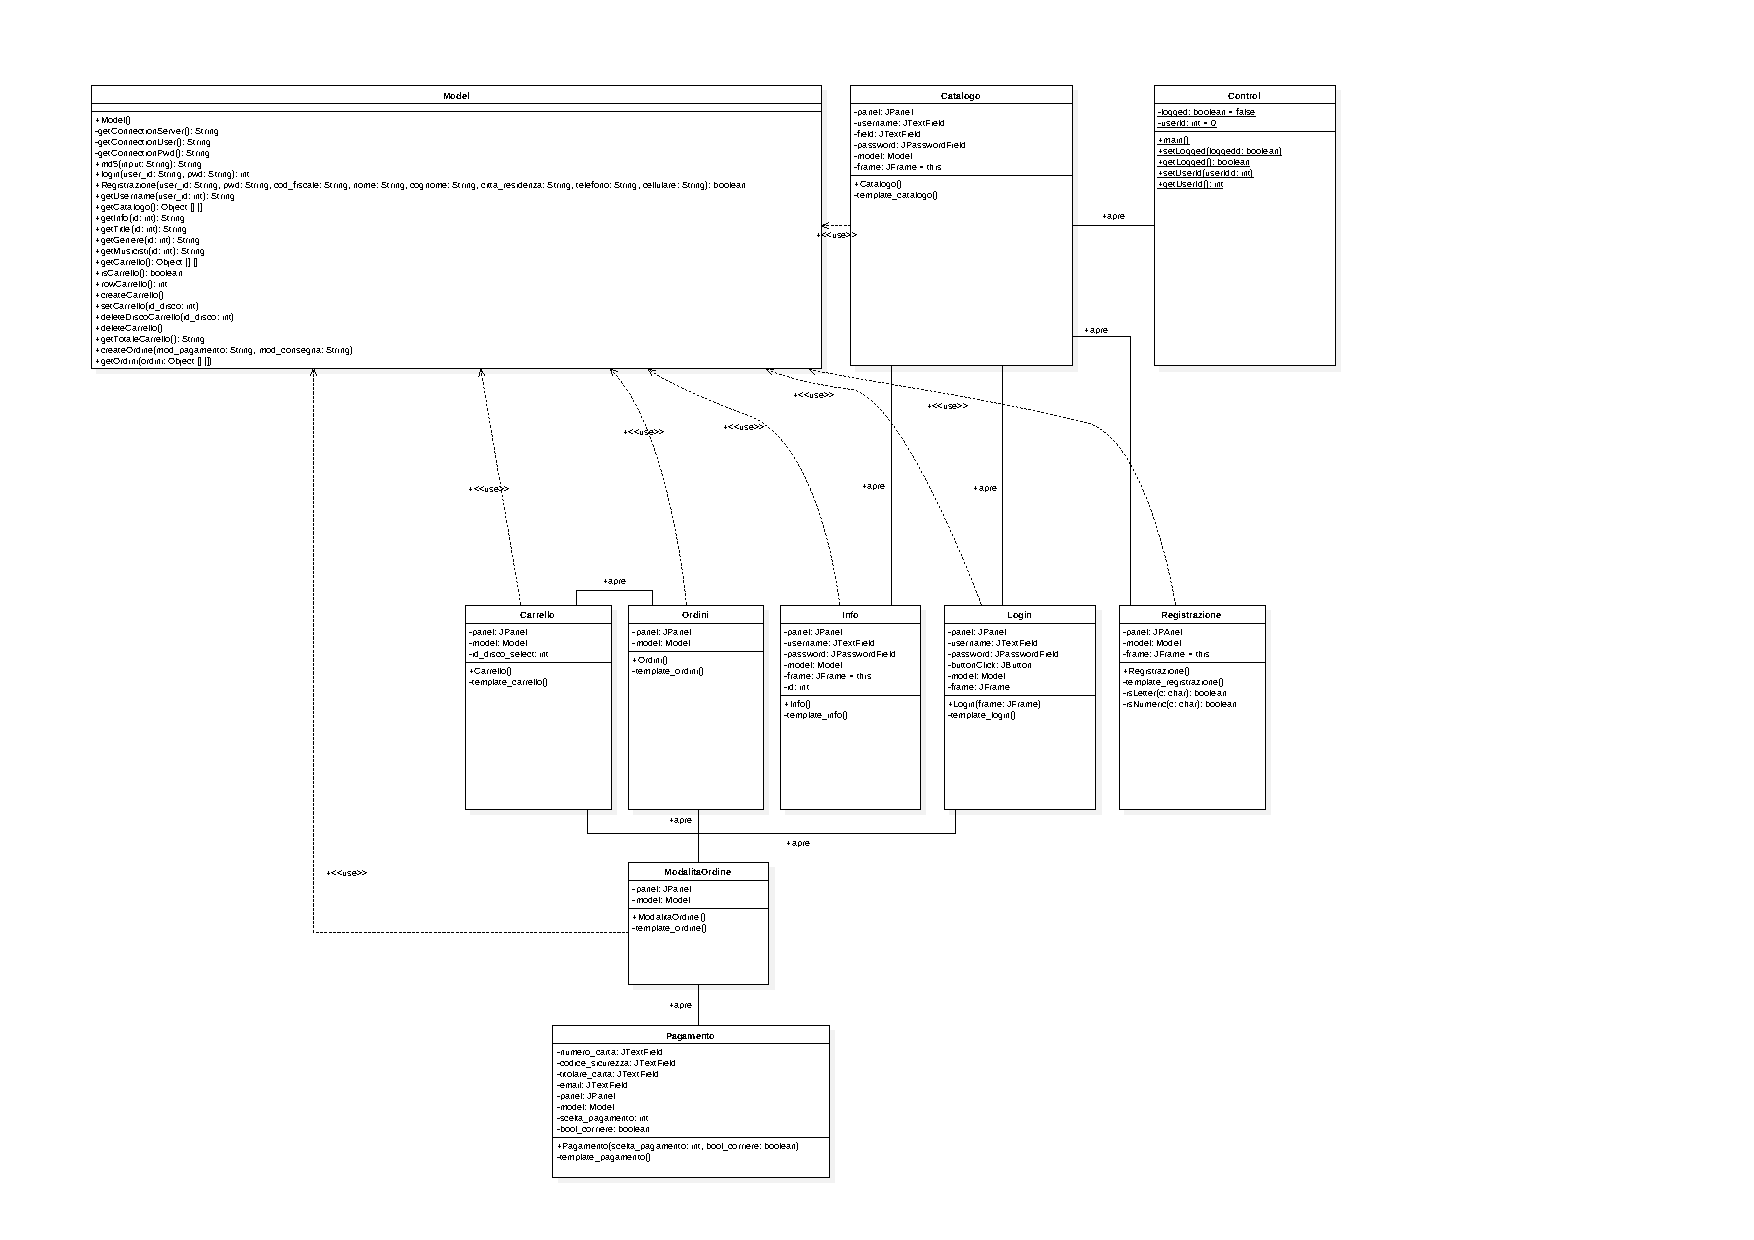
\includegraphics[width=450px]{img/Class.pdf}
\caption{Class Diagram \label{fig:cla}}
\end{figure}

\section{Entity-relationship Diagram}
\begin{figure}[H]
\center
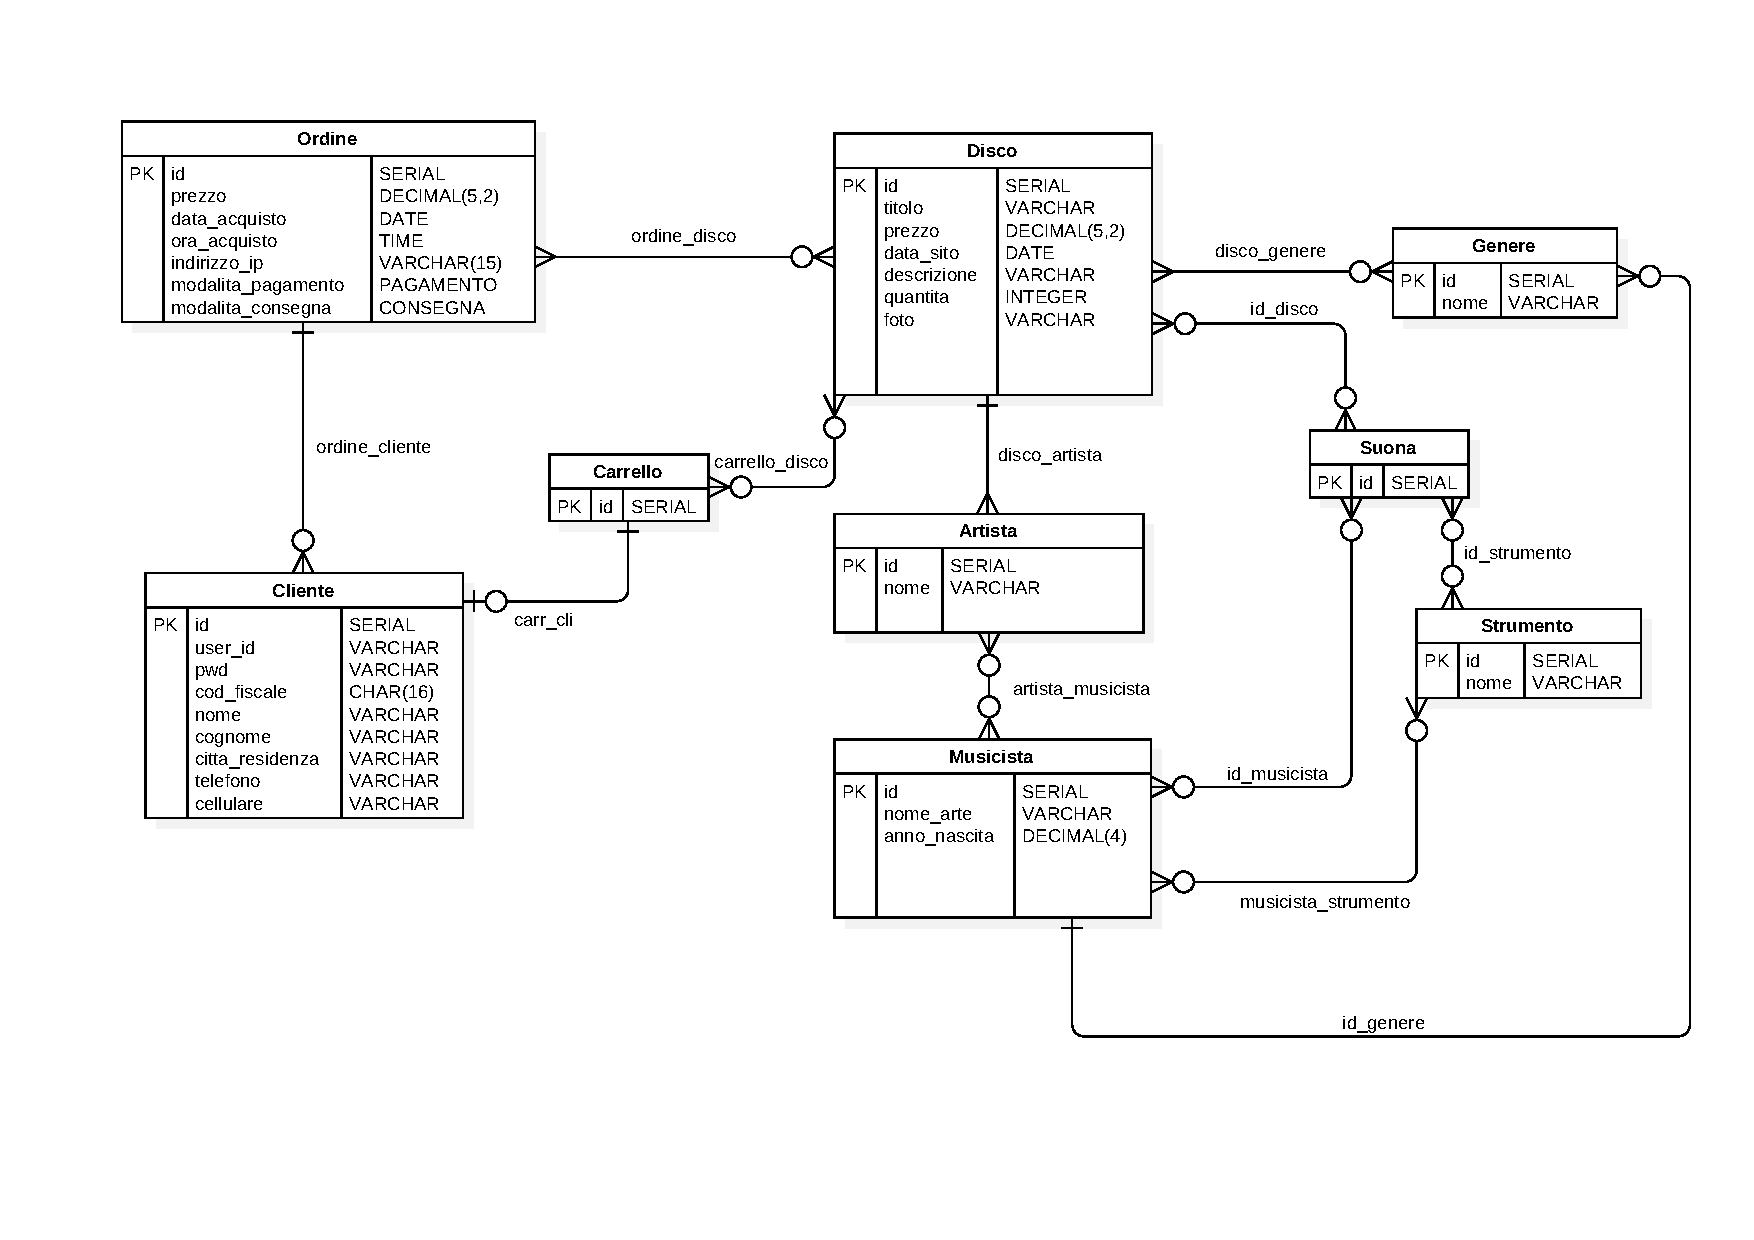
\includegraphics[width=350px]{img/ERD.pdf}
\caption{Database \label{fig:cla}}
\end{figure}

\backmatter
\bibliography{biblio}
\bibliographystyle{plain}

\nocite{ingsft}
\nocite{ingreq}
\nocite{inglab}

\end{document}